% !TeX program = pdflatex
% !BIB program = biber
% !IDTX program = makeglossaries
\documentclass[a4paper,11pt,onecolumn]{article}

% --------------------------------------------------------
% Encoding & Language
% --------------------------------------------------------
\usepackage[utf8]{inputenc}
\usepackage[T1]{fontenc}
\usepackage{float}
\usepackage{booktabs}
\usepackage{tabularx}
\usepackage[english]{babel}

% --------------------------------------------------------
% Template variables
% --------------------------------------------------------
\newcommand{\TitleSealFile}{logos/Newcastle.png}
\newcommand{\TitleSealWidth}{0.5\textwidth}
\newcommand{\ThesisTitle}{Design and Evaluation of an Accessible IDE Plugin for Supporting Neurodivergent Software Developers}
\newcommand{\ProgramName}{Computer Science}
\newcommand{\SupervisorName}{Dr. Vlad Gonzalez}
\newcommand{\AuthorName}{Clo Elis}
\newcommand{\StudentNumber}{220402088}
\newcommand{\SubmissionMonth}{May}
\newcommand{\SubmissionYear}{2026}

% --------------------------------------------------------
% Fonts & Spacing
% --------------------------------------------------------
\usepackage{newtxtext,newtxmath}
\usepackage[top=2.5cm,bottom=2cm,inner=4cm,outer=2cm]{geometry}
\usepackage{setspace}
\onehalfspacing
\usepackage{footmisc}
\setlength{\footnotesep}{0.8\baselineskip}
\renewcommand{\footnotelayout}{\setstretch{1.0}}

% Packages
\usepackage{amsmath, graphicx, url, xcolor, csquotes, etoolbox}
\AtBeginEnvironment{table}{\singlespacing}
\urlstyle{rm}

% --------------------------------------------------------
% Hyperlinks
% --------------------------------------------------------
\usepackage[pdfpagelabels,plainpages=false,hypertexnames=false]{hyperref}
\definecolor{smdsblue}{RGB}{0,69,134}
\hypersetup{
    colorlinks=true,
    linkcolor=black,
    citecolor=black,
    urlcolor=smdsblue
}

% --------------------------------------------------------
% Bibliography & Glossaries
% --------------------------------------------------------
\usepackage[backend=biber,maxcitenames=2,maxbibnames=99,natbib=true]{biblatex}
\addbibresource{references.bib}

% Using 'abbreviations' type for better separation
\usepackage[acronym, toc, nohypertypes={main,acronym}]{glossaries}
\makeglossaries%
% --- ABBREVIATIONS ---
\newacronym[longplural={Large Language Models}]{LLM}{LLM}{Large Language Model}
\newacronym[longplural={Integrated Development Environments}]{IDE}{IDE}{Integrated Development Environment}
\newacronym{ADHD}{ADHD}{Attention-Deficit/Hyperactivity Disorder}
\newacronym{ASD}{ASD}{Autism Spectrum Disorder}
\newacronym{AI}{AI}{Artificial Intelligence}
\newacronym{NASATLX}{NASA-TLX}{NASA Task Load Index}
\newacronym{SUS}{SUS}{System Usability Scale}
\newacronym{WCAG}{WCAG}{Web Content Accessibility Guidelines}
\newacronym{CoT}{CoT}{Chain of Thought}
\newacronym{HITL}{HITL}{Human-in-the-Loop}
\newacronym{API}{API}{Application Programming Interface}
\newacronym{UI}{UI}{User Interface}

% --- GLOSSARY ENTRIES ---
\newglossaryentry{neurodivergent}{
    name=neurodivergent,
    description={A term used to describe people whose brains function, learn, and process information differently than what is considered typical}
}
\newglossaryentry{executive_dysfunction}{
    name=executive dysfunction,
    description={A range of cognitive difficulties affecting the ability to plan, focus attention, and multi-task}
}
\newglossaryentry{hyperfocus}{
    name = hyperfocus,
    description = {}
}
\newglossaryentry{Dyslexia}{
    name = Dyslexia,
    description = {}
}
\newglossaryentry{task_paralysis}{
    name = task paralysis,
    description = {}
} % Ensure this file contains your entries
% Formatting
\parindent0em
\parskip6pt
\usepackage{tocloft}
\setlength{\cftbeforesubsubsecskip}{1pt}
\setlength{\cftbeforetabskip}{3pt}

% --------------------------------------------------------
% Main document
% --------------------------------------------------------
\begin{document}

% 1. Title Page
\newgeometry{ top=2.5cm, bottom=2cm, left=3cm, right=3cm }

\begin{titlepage}
\begin{center}
\vspace*{\fill} % oben strecken
\begin{minipage}{0.9\textwidth}
\begin{center}
\setstretch{1.5} % Zeilenabstand 1,5

% Uni Logo
\IfFileExists{\TitleSealFile}{%
  \includegraphics[width=\TitleSealWidth]{\TitleSealFile}\par\vspace{0.8cm}%
}{%
  \PackageWarning{template}{Seal logo file not found: \TitleSealFile}%
}

\large\textbf{\ThesisTitle}\\[1.2cm]
\AuthorName \\
\StudentNumber\\
\SubmissionMonth\ \SubmissionYear\\
[0.8cm]


\ProgramName\\
Supervisor: 'I\&'\SupervisorName\\

\vspace{1.5cm}
\vfill
\end{center}
\end{minipage}
\vspace*{\fill}
\begin{center}


\end{center}
\end{center}
\end{titlepage}

\restoregeometry
\glsaddall
% 2. Front Matter (Roman)
\pagenumbering{Roman}

\section*{Abstract}
Modern Integrated Development Environments~(\glspl{IDE}) prioritise feature density, often at the expense of cognitive accessibility. 
For \gls{neurodivergent} software developers, particularly those with Attention-Deficit/Hyperactivity Disorder~(\gls{ADHD}), Autism Spectrum Disorder~(\gls{ASD}), or \gls{dyslexia} this complexity manifests as 
significant barriers driven by \gls{executive_dysfunction}, including cognitive overload and difficulty in \gls{task_initiation}. 
This research investigates the efficacy of an Artificial Intelligence~(\gls{AI}) integrated plugin designed to mitigate these challenges within the VS Code 
ecosystem.


The developed solution comprises three core modules: a toggle to close all unnecessary panels to filter interface-driven distractions, 
a task breakdown tool to leverage Large Language Models~(\gls{LLM}) to decompose complex requirements into structured checklists, 
and a visual styling tool for high-contrast, low-strain environmental presets. The system's impact was evaluated through a comparative
 user study ($N=5$) pitting a standard VS Code baseline against the enhanced environment. Evaluation metrics included the 
NASA Task Load Index~(\gls{NASATLX})~\cite{NASATLX} to quantify shifts in mental workload and the System Usability Scale~(\gls{SUS})~\cite{Hyzy2022} to assess overall usability 
 and tool effectiveness.
 
 Results indicate that by streamlining the development environment and providing automated task \gls{scaffolding}, 
 the plugin significantly reduces the executive tax imposed by standard tools. This allows \gls{neurodivergent} developers to 
 reallocate critical cognitive resources from interface navigation to core algorithmic problem-solving.
\addcontentsline{toc}{section}{Abstract}
\clearpage

\textbf{Declaration}
“I declare that this document represents my own work except where otherwise stated” - Clo Ellis

\textbf{Acknowledgments}
I would like to express my sincere gratitude to my supervisor, Dr. Vlad Gonzalez, for his guidance and support throughout this project. 
I also want to thank all the participants who contributed to this study, without whom this work would not have been possible.
\clearpage

\tableofcontents
\clearpage

% 3. Lists (Abbreviations & Glossary)
\printglossary[type=\acronymtype, title={List of Abbreviations}]
\clearpage

\printglossary[title={Glossary}]
\clearpage

% 4. Main Body (Arabic)
\pagenumbering{arabic}
\section{Introduction}
\subsection{Motivation}
This project was initially motivated by my lived experience as a \gls{neurodivergent} developer. In professional settings, \gls{ASD} is frequently 
romanticised as a ``superpower'' due to the high capacity for deep logical analysis
and rapid skill acquisition. However, this perceived strength came with a significant \gls{cognitive_tax}. Adapting to new environments, fluctuating workloads and 
maintaining a sustainable work-life balance is often extremely difficult as current tools like \glspl{IDE} lack out of the box features to mitigate 
these executive functioning barriers. This research seeks to transition the \gls{IDE} from a passive tool into an active cognitive partner through AI-driven support.


\subsection{Problem Statement}
While modern \glspl{IDE} are feature-rich, their design reflects a \gls{neurotypical-bias} that assumes a high baseline for filtering sensory input and managing 
multi-step planning. For developers with \gls{ADHD}, \gls{ASD}, or \gls{Dyslexia}, these tools often exacerbate Extraneous Cognitive Load, 
the mental effort spent on processing the interface rather 
than the problem logic~\cite{sweller1988cognitive}.

Current \glspl{IDE} prioritise feature density, often resulting in visual noise from nested menus and persistent notifications. Research indicates that developers with \gls{ADHD} 
frequently experience \gls{task_paralysis}, difficulty initiating tasks during a project~\cite{bramham2009executive}, while those with \gls{ASD} may struggle with the \gls{double_empathy} problem, leading to them misinterpreting 
ambiguous or implied requirements from team members~\cite{Milton01102012}. Existing AI tools focus almost exclusively on code generation rather than process support. Consequently, there is a critical need 
for an \gls{IDE} intervention that acts as a digital ramp, filtering noise and providing the scaffolding necessary to bypass the executive freeze response.

\subsection{Understanding \Gls{neurodiversity} in Software Development}
Before going into the specific technical barriers of modern \glspl{IDE}, it is necessary to define \gls{neurodiversity} and the cognitive
 frameworks that underpin this research. Originally coined by Judy Singer in the late 1990s, \gls{neurodiversity} views neurological differences, such 
 as \gls{ASD}, \gls{ADHD}, and \gls{Dyslexia}, as natural variations in the human genome rather than purely medical deficits~\cite{singer1999why}.

In the context of software engineering, these variations often manifest as unique cognitive processing styles. While many \gls{neurodivergent} 
developers possess high aptitude for logic and pattern recognition, they frequently encounter barriers related to \gls{executive_dysfunction}. 
This is an umbrella term for difficulty in mental processes that enable us to plan, focus attention, remember instructions, and juggle multiple tasks 
successfully. For a developer, \gls{executive_dysfunction} is not a lack of technical ability, but rather a barrier in three key areas: Inhibitory Control
 (filtering \gls{IDE} distractions), Working Memory (tracking complex syntax), and Cognitive Flexibility (switching between high-level logic and low-level code).

To provide a clearer lens for the objectives of this project, the below table outlines the specific strengths and environmental challenges associated with the conditions most prevalent in the developer community~\cite{sperry2005perceptions}~\cite{hotte2024strengths}~\cite{roitsch2019overview}.
\begin{table}[H]
    \centering
    \caption{\Gls{neurodivergent} Strengths and Environmental Challenges}
    \renewcommand{\arraystretch}{1.5} % Adds breathing room between rows
    \begin{tabularx}{\textwidth}{l >{\raggedright\arraybackslash}X >{\raggedright\arraybackslash}X}
        \toprule
        \textbf{Condition} & \textbf{Potential Strengths} & \textbf{Common Environmental Challenges} \\
        \midrule
        \gls{ASD} & Deep focus, systematic thinking, high integrity, exceptional memory for details, strong pattern recognition. & Sensory overload in noisy or bright environments, misinterpretation of direct communication style, difficulty with unspoken social rules. \\
        \addlinespace
        \gls{ADHD} & Creativity, hyperfocus on passions, adaptability, high energy, ability to multitask or rapidly switch contexts. & Distractibility in chaotic settings, struggles with time management and organisation leading to \gls{time-blindness} and issues with task initiation, impulsivity in structured environments.\\
        \addlinespace
        \gls{Dyslexia} & Strong visual-spatial reasoning, excellent big-picture thinking, creative problem-solving, strong verbal skills. & Difficulties with text-heavy tasks, timed reading assignments, and conventional written communication. \\
        \bottomrule
    \end{tabularx}
\end{table}

\subsection{Aims and Objectives}

\subsubsection{Project Aim}

The primary objective of this project is to design, implement, and evaluate an assistive VS Code plug-in that reduces extraneous cognitive load and mitigates the effects of
 \gls{executive_dysfunction} for \gls{neurodivergent} software developers. By introducing a cognitive prosthetic layer, the project seeks
  to determine if targeted \gls{UI} simplification and \gls{AI}-driven task scaffolding can measurably improve the developer experience.

\subsubsection{Research Objectives}

\textbf{Objective 1:} Interface Optimisation (The Minimalist Toggle)

Target: Develop a single ``Minimalist Toggle'' feature that simultaneously hides non-essential \gls{UI} elements, including the Activity Bar, Status Bar, Mini-map, and Breadcrumbs.


Justification: This directly addresses the issue of visual overload by reducing the number of stimuli competing for the developer's attention, thus lowering the Extraneous
 Cognitive Load and creating a more focused coding environment \cite{sweller1988cognitive}, reducing visual noise that leads to distraction and sensory overwhelm for autistic and \gls{ADHD} developers.

\textbf{Objective 2: }\gls{AI}-Driven Task Decomposition (The Task Architect)

Target: To implement an \gls{LLM}-integrated module that translates ambiguous programming goals into structured, editable checklists using a Chain of Thought (CoT) prompting strategy. This should be
implemented via the Open\gls{AI} \gls{API} that breaks down high-level requirements~\cite{ringel2019ai}.


Justification: This supports task initiation and reduces the energy required to overcome task paralysis, a primary barrier for developers with \gls{ADHD} and \gls{ASD}~\cite{gama2025socio}.

\textbf{Objective 3:} Simplification of Technical Feedback (The Code Explainer)

Target: To build a diagnostic interceptor that re-interprets complex compiler errors into plain-language, bulleted instructions~\cite{rocha2025conceptual}. Limit output to a maximum of three bullet points using direct instructions style.


Justification: This minimizes the cognitive demand of interpreting dense jargon, preventing rabbit holes and supporting the literal communication needs identified in the Double Empathy
 problem. By simplifying the feedback loop, developers can maintain focus on the core problem rather than getting lost in peripheral details. This is particularly beneficial for those with \gls{ASD},
  who may struggle with implied logic and prefer clear, direct instructions. Additionally, it can help mitigate the hyperfocus trap by providing concise guidance that keeps the developer on track 
  without overwhelming them with information.

\textbf{Objective 4: }Visual Accessibility Customisation (The Visual Styler)

Target: To create at least two visual presets, such as ``Soft High Contrast'', that adhere to \gls{WCAG} 2.1, set of international standards designed to make web content more accessible to people with disabilities it can also help with visual processing, eye strain and enhance readability~\cite{bengtsson2025web}.

Justification: Addresses the sensory sensitivities and colour preferences reported by \gls{neurodivergent} developers in research surveys~\cite{rocha2025conceptual}.

\textbf{Objective 5:} Empirical Evaluation of Cognitive Impact

Target: To conduct a comparative study using the \gls{NASATLX} and the \gls{SUS} to validate the plugin's efficacy against a standard \gls{IDE}.

Justification: This provides a standardized scientific metric to confirm if the tool successfully reduces mental demand and frustration for the target demographic.

\subsection{Dissertation Structure}

This dissertation is organized into five sections, following a logical progression from theoretical grounding to empirical validation:
\begin{itemize}
  \item \textbf{Section 2: Literature Review} I will evaluate the foundational psychological frameworks of Cognitive Load Theory (CLT) and Multimedia Learning (CTML). This provides a theoretical foundation for other research into the current state of \gls{neurodivergent} 
  software engineering as well as the shift toward a more social model of disability rather than a medical model.
  \item \textbf{Section 3: Design and Implementation} Details the user requirements and the three-layer system architecture. This chapter explains the technical
   execution of ``Minimalist Toggle'' and ``Task Architect'' as well as the visual presets and styling tools. I will also discuss issues encountered during development and how they were resolved, such as the design of the UI and issues with the AI integration and prompt generation.
  \item \textbf{Section 4: Results and Discussion} Presents the quantitative and qualitative findings from the user study ($N=5$). It analyzes the 82\% reduction in perceived workload measured by the NASA-TLX 
  and evaluates the tool`s excellent usability rating via the System Usability Scale (SUS). This section also includes a critical discussion of the results, exploring the implications for future assistive 
  technology in software development and acknowledging the limitations of the study, such as the small sample size and potential biases in participant selection.
  \item \textbf{Section 5: Conclusion} Summarises the core findings, acknowledges research limitations, and proposes specific avenues for future work with larger, more diverse participant pools.
\end{itemize}

\newpage
\section{Literature Review}
\subsection{Cognitive Load Theory (CLT)}
Cognitive Load Theory, primarily developed by John Sweller, suggests that since the human brain has limited \gls{working_memory} capacity, instructional design can aid in avoiding overload.
\textcite{sweller1988cognitive} proposes a three-part load framework that identifies three different types of cognitive load that impact a learner's ability to process information:

\begin{enumerate}
    \item Intrinsic Load~(\gls{IL}): This is the inherent difficulty of the task itself. It is defined by the number of elements must be processed 
    simultaneously to understand a concept. For example, learning basic vocabulary has low \gls{IL}, while mastering complex syntax has high \gls{IL}.
    \item Extraneous Load~(\gls{EL}): This is seen as the unnecessary load that you would aim to minimise wherever possible. It is influenced by the way 
    information is presented. Some examples that could exacerbate the load are poorly designed diagrams, distracting environments or redundant
     text. Poor design choices force the brain to waste resources on non-essential processing.
    \item Germane Load~(\gls{GL}): This is the load I am aiming to maximise. It refers to the mental effort that can be directed toward the more key task, 
    which in this scenario would be the code programming task.
\end{enumerate}

The framework can be simplified down to the idea that the Total Cognitive Load~(\gls{TCL}) is the sum of \gls{IL}, \gls{EL}, and \gls{GL}. 
The goal of instructional design is to manage these loads effectively to maximise learning outcomes.
$$TCL = IL + EL + GL$$

\begin{figure}[H]
    \centering
    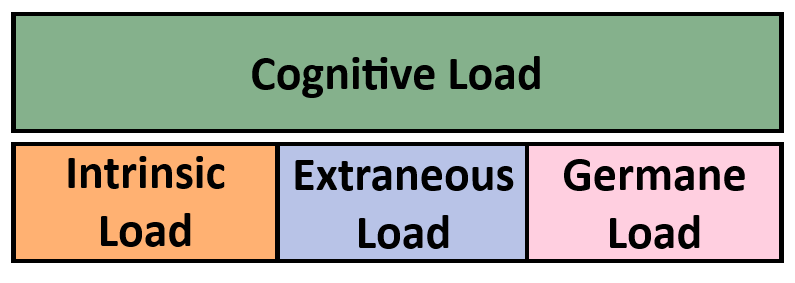
\includegraphics[width=0.8\linewidth, alt={A diagram illustrating Sweller's Tripartite Model. It shows Total Cognitive Load as a header, supported by three equal categories: \gls{IL} (task difficulty), \gls{EL} (presentation noise), and \gls{GL} (knowledge construction).}] {logos/clt_diagram.png}
    \caption{Sweller's Tripartite Model of Cognitive Load, illustrating the balance between Intrinsic, Extraneous, and Germane loads.}\label{fig:clt_diagram}
\end{figure}

While Sweller's Cognitive Load Theory provides the theoretical foundation, the application of these principles to \gls{neurodivergent} developers requires 
a more nuanced approach. One of the main focuses of this project is that for these developers, the \gls{IDE} environment often imposes a 
disproportionate \gls{EL}. When \gls{EL} is high, the cognitive budget is exhausted before the developer can engage with the core logic of the code, leading to \gls{task_paralysis}. 
My plugin aims to free up this mental bandwidth by suppressing \gls{EL} (via the Minimalist Toggle) and \gls{scaffolding} \gls{IL} (via the Task Architect),
thereby maximising the availability of cognitive resources for Germane processing. By reducing the noise and providing structured support, the plugin allows \gls{neurodivergent} developers to focus
their cognitive resources on the actual problem-solving aspect of programming, rather than being overwhelmed by the interface or the complexity of the task at hand.

\subsection{Applying CLT to \Gls{neurodiversity}}
For \gls{neurodivergent} developers, the \gls{EL} is not just due to bad design, but a barrier to entry. Features like the Activity Bar and Mini-map, while useful for some, can
be filtered out by a neurotypical developer but act as visual noise for those with \gls{ADHD} or \gls{ASD}.
To be able to code a high \gls{IL} is required. However, if the activation energy to start is too high due to \gls{executive_dysfunction}, the developer 
never reaches the stage where they can handle that load.
Having a single switch that closes all UI elements will directly targetC the suppression of \gls{EL} to free up mental bandwidth instantly without having to navigate menus.
While the \gls{AI} task decomposition tool acts as a cognitive prosthetic that scaffolds the \gls{IL} of project planning, preventing \gls{task_paralysis}.


\subsubsection{Integration with Rosenshine`s Principles of Instruction}

While Sweller provided the theoretical framework, Barack Rosenshine provided a \textit{how-to} to be used in classrooms or digital 
environments~\cite{rosenshine2012principles}. 

Main connections to Sweller`s principles include:

\begin{itemize}
    \item Small Steps (Principle 2): By presenting new material in small increments, the instructor limits the \gls{IL}, ensuring the 
    \gls{working_memory} is not overwhelmed at the outset.
    \item \Gls{scaffolding} (Principle 7): Providing temporary supports reduces \gls{EL}, allowing the learner to focus their cognitive 
    resources on the core task rather than the noise of the process.
\end{itemize}

To view these from more of a development lens, principle 2 supports breaking down the core task into smaller, more manageable steps. 
Further more these smaller task can be seen as \gls{scaffolding} for the user when they are beginning a task without handing them the answer directly.


\subsubsection{The Cognitive Theory of Multimedia Learning (CTML)}
While Sweller’s Cognitive Load Theory focuses primarily on the nature and management of cognitive load, Mayer`s \gls{CTML}~\cite{mayer2005cognitive} 
provides a more detailed explanation of how information is processed across visual and auditory channels. Within the context of software development, the
\gls{IDE} can be understood as a high-density multimedia environment in which multiple streams of related information must be processed simultaneously.

Within this framework, Ayres and Sweller`s split-attention principle describes the split-attention effect as occurring when learners are required to divide their attention 
between physically separated yet cognitively related sources of information~\cite{AyresSweller2021}. In a software development context, this may occur when an error message 
in the console refers to a line of code located hundreds of lines away in the editor. For a \gls{neurodivergent} developer, this creates a significant spatial split, requiring 
additional mental effort to navigate between and mentally integrate these sources of information. This integration process contributes directly to extraneous cognitive load, 
as cognitive resources are expended on locating and connecting information rather than resolving the underlying programming problem.

To mitigate this, the plugin`s \textit{Code Explainer} feature will provide an integrated view that combines the error message with the relevant code context, effectively 
reducing the split-attention effect. By presenting the error message and the associated code in a unified interface, the plugin minimises the need for mental integration
 across separate sources, thereby reducing extraneous cognitive load and allowing developers to focus more effectively on problem-solving.


\subsection{\Gls{neurodiversity} in Software Engineering}
To best design an inclusive plug-in, I needed to gain a deep understanding of the specific cognitive roadblocks faced by \gls{neurodivergent}
 developers. Recent research by \textcite{verma2025differences} and \textcite{gama2025socio} highlights that developers with \gls{ADHD}, 
 \gls{ASD}, and \gls{dyslexia} face significantly higher frequency of interruptions and difficulty obtaining knowledge.

\subsubsection{The Cognitive Load Connection}

For a \gls{neurodivergent} developer, a standard \gls{IDE} error message often carries a high \gls{EL}. What a neurotypical developer
 might perceive as a simple notification, a \gls{neurodivergent} individual may experience as a wall of cryptic text, inconsistent highlighting, 
 and ambiguous phrasing. This noise competes for limited \gls{working_memory} resources, leaving little room for the \gls{IL} required actually 
 to solve the logical problem.

\subsubsection{Executive Functioning and Task Switching}

\Gls{executive_dysfunction} is a primary barrier cited by both~\textcite{verma2025differences} and~\textcite{gama2025socio}. This manifests
 itself as difficulty in \gls{task_initiation} (starting a new project) and switching between tasks.

\textbf{The Industry Context:} In a modern software environment, developers are rarely afforded the luxury of a single focus; they must
 balance code reviews, meetings, and multiple projects.

\textbf{The Impact:} For those with \gls{ADHD}, the mental cost of having to remember the context of a project after an interruption is significantly higher. If the \gls{IDE} does not provide clear "waypoints" or historical context, the developer may become cognitively paralysed, unable to determine where they left off.

\subsubsection{Specific Challenges by Condition}

Based on the synthesis of recent studies, the challenges can be categorised as follows:

\textbf{\gls{ADHD}}: Frequent loss of state due to external interruptions and internal distraction.\textcite{verma2025differences} found that these developers report higher stress related to waiting for answers, as delays in information retrieval often lead to a total loss of task momentum.

\textbf{\gls{ASD}}: Challenges with the \Gls{double_empathy} problem in code, where the high-level abstractions or implied logic used by neurotypical colleagues create a high cognitive overhead for autistic developers who prefer explicit, literal documentation.

\textbf{\Gls{dyslexia}}: Significant hurdles during the syntax-heavy stages of programming. While these developers often excel at high-level architectural mapping, the \gls{EL} of spelling-sensitive compiler errors and dense documentation can be a major deterrent to productivity.

\subsubsection{Beyond Medical}

To understand why existing tools fail, we  must examine the shift from the \Gls{medical_model} to the \Gls{social_model}.

\begin{itemize}
    \item \textbf{The \Gls{medical_model}}: Traditionally, \gls{ADHD} or \gls{dyslexia} in engineering has been viewed as a deficit to be corrected through individual coaching or medication.
    \item \textbf{The \Gls{social_model}}: This perspective argues that the developer is disabled not by their neurology, but by an \gls{IDE} designed with a \gls{neurotypical-bias}. The problem is not the individual's
     brain, but the environment that fails to accommodate it. This shift in perspective is crucial for designing tools that are not just assistive but truly inclusive, as it focuses on modifying the
      environment (the \gls{IDE}) rather than trying to fix the individual.
\end{itemize}

The minimalist toggle and the code explainer are designed with this \gls{social_model} in mind, aiming to create an environment that reduces barriers and allows \gls{neurodivergent} developers to thrive 
without needing to conform to a neurotypical standard.

\Gls{EF} Domains in Programming
To deepen the analysis of \gls{executive_dysfunction}, we must break it into three core domains:
\begin{itemize}
    \item \textbf{Inhibitory Control}: The ability to ignore distractions. For \gls{ADHD} developers, the \textit{pop-up} notifications of a linter can break a fragile state of focus.
    \item \textbf{\Gls{working_memory}}: Dyslexic developers often have a high capacity for 3D spatial reasoning but a limited verbal \gls{working_memory}, making syntax-heavy languages like C++ more taxing than cleaner languages like Python.
    \item \textbf{Cognitive Flexibility}: The ability to switch between thinking about the big picture architecture and the low-level syntax.
\end{itemize}

\subsubsection{The Double-Edged Sword of \Gls{hyperfocus}}
While \gls{neurodivergent} developers, particularly those with \gls{ASD} and \gls{ADHD}, are often stereotyped as having a \textit{superpower} for deep work, 
this ability to \gls{hyperfocus} is more accurately described as a dysregulation of attention. Unlike the psychological concept of \textit{flow} which is
 generally sustainable and self-directed, \gls{hyperfocus} is an involuntary immersion into a task or activity. As noted by~\textcite{gama2025socio}, \gls{hyperfocus} allows 
for an exhaustive exploration of complex problems, yet this intensity often comes at the expense of self-care. Developers may neglect fundamental 
biological needs, such as nutrition, sleep, and hygiene, leading to rapid burnout. 

In the context of software engineering, this creates a High-Intensity/High-Fragility paradox.~\textcite{newman2025get} identifies that for \gls{ADHD} programmers, achieving a flow state is a fragile process where a single interruption can collapse hours of built-up mental context. The subsequent \gls{state_recovery_cost} is significantly higher 
for \gls{neurodivergent} individuals, often leading to burnout or irritability when the state is broken.

In a professional engineering context, this creates a significant conflict between depth and delivery. \Gls{hyperfocus} can inadvertently trigger over-engineering, 
where a developer becomes locked into optimising a single component while neglecting broader project milestones or team collaborations. This inability to switch 
off from an interesting problem makes task-switching, a fundamental requirement of agile development, mentally exhausting and practically difficult. Consequently, 
what appears to be peak productivity from the outside is often an unsustainable trade-off that risks both the developer's well-being and the project's timeline.

\subsection{Existing Tools}
The design of \glspl{IDE} often follows a one-size-fits-all model, which inherently leads to a \gls{neurotypical-bias}, creating barriers for those who may 
require additional support.~\textcite{morris2015understanding} observes workplace tools are frequently built with assumptions that ``may not align with 
the needs of \gls{neurodiverse} employees.'' \glspl{IDE} are often packed with tools that enable customisation; however, they are not designed with \gls{neurodiverse} 
developers in mind, and complex nested menus can be overwhelming.

Despite the obstacles described, certain features provide essential support for developers.~\textcite{morris2015understanding} notes that tools such as code 
completion and linters are vital to alleviate the difficulties associated with \gls{dyslexia}, such as syntax memorisation and spelling.

However, the burden of making tools accessible often falls to the user.~\textcite{liebel2024challenges} found that developers often create ``individual
 strategies and tool configurations to support their productivity''. While these features are currently helping, the reliance on manual customisation 
 implies a lack of \textit{out-of-the-box} inclusivity.

This project aims to bridge the gap between the availability of generic tools and their functional utility. While current tools are excellent at
 detecting errors, they often fail at explaining them in an accessible manner. By integrating an Error Explainer that decomposes complex compiler 
 messages into manageable tasks, therefore reducing the cognitive load required to debug. This shifts the \gls{IDE} from a passive environment that 
 requires expert configuration to an active partner in the development process.

\subsection{Pomodoro Timer}
The Pomodoro Technique, developed by Francesco Cirillo~\cite{cirillo2018pomodoro} in the late 1980s, is a time-management framework that partitions work into focused intervals. Typically
25 minutes, separated by brief five-minute breaks. In the context of \gls{neurodiversity}, this method is often reframed as a cognitive tool rather than a rigid 
rule set, specifically designed to address common \gls{EF} barriers~\cite{miller2025wired}.

\subsubsection{Managing \Gls{executive_dysfunction} and \Gls{task_paralysis}}
For developers with \gls{ADHD} or \gls{ASD}, \gls{task_paralysis}, an inability to initiate work due to cognitive overload or anxiety represents a significant hurdle. 
The Pomodoro Technique mitigates this by lowering the activation energy required to start. By committing to a manageable, 25-minute sprint, the psychological 
barrier to entry is reduced, helping individuals bypass the freeze response associated with daunting or abstract tasks.

\subsubsection{Combatting \Gls{time-blindness} and \Gls{hyperfocus} Burnout}
\Gls{neurodivergent} individuals often experience \gls{time-blindness}, a difficulty in perceiving the passage of time as a concrete resource. Externalising time through a visual 
or auditory timer provides real-time feedback, helping to anchor the developer to the present task and reducing the risk of underestimating project timelines.

Furthermore, while \gls{hyperfocus} can lead to severe mental and physical exhaustion if left unregulated. The structured 
nature of the Pomodoro cycle acts as a release valve for focus:
\begin{itemize}
\item Mandatory Breaks: Frequent breaks prevent the \gls{hyperfocus} trap, where a developer may neglect basic biological needs like nutrition or hydration.

\item Sensory Regulation: Scheduled pauses provide essential space for sensory recovery, allowing developers to move around to prevent the physical strain and irritability that often follow hours of sedentary deep work.
\end{itemize}

\subsubsection{Cognitive Load and Adaptive Implementation}
From the perspective of Cognitive Load Theory (CLT), the Pomodoro Technique manages mental resources by preventing the exhaustion of the cognitive budget. By breaking a 
complex project into small, time-limited stages, the method reduces \gls{EL}, the unnecessary effort required to manage a vast, unstructured task, allowing for more 
\gls{GL} to be directed toward core algorithmic problem-solving.

However, In some cases it could be argued that the standard Pomodoro settings can sometimes be counterproductive if applied too rigidly. For individuals with \gls{ADHD}, 
a 25-minute window may be too short to enter a productive flow state, leading to \glspl{state_recovery_cost} if interrupted too early. To address this, the plugin
 will allow users to customise the length of their focus intervals and breaks, providing flexibility to accommodate different working styles and cognitive needs.

\subsection{Colour filters}
Visual presentation can influence reading performance and comfort.~\textcite{griffiths2016effect} found that coloured overlays may reduce visual stress for some readers, 
although the benefits vary significantly between individuals. This suggests that software tools should support flexible visual customisation rather than relying on a single accessibility configuration.

In some cases, high-contrast models are essential because they provide the necessary visual \gls{scaffolding} to combat \gls{task_paralysis}. For developers with \gls{ADHD}, a low-contrast or pastel theme can
cause code elements to bleed together, increasing the cognitive effort required to distinguish between keywords, variables, and logic.
By utilising high-contrast ratios such as 7:1 or higher, per \gls{WCAG} 2.1 guidelines the \gls{IDE} creates a clear visual hierarchy.

This high signal environment provides several technical advantages:
\begin{itemize}
    \item Reduce Visual Search Time: Finding the start and end of a function block becomes instantaneous rather than a manual scan.
    \item Mitigate the Blur of \Gls{hyperfocus}: As noted by~\cite{newman2025get}, the intense mental strain of being in the groove can lead to visual fatigue; high contrast maintains legibility even as physiological focus wanes.
    \item Support Syntax Logic: In complex, nested code, high-contrast separation between brackets and operators serves as a visual prosthetic, offloading the work of pattern recognition from the brain to the interface.
\end{itemize}

\subsubsection{The \Gls{halation} Risk and Soft High Contrast}
While high contrast is vital for clarity, pure high contrast (e.g., stark white text on a pure black background) can be counterproductive for those with \gls{ASD} or specific visual stresses.
 This combination can cause \gls{halation}, a glowing or bleeding effect around letters that makes text appear to vibrate or move~\cite{cruz2025empiricalinvestigationexperiencesdyslexic}.

 To address this, the most effective models for \gls{neurodiversity} are often \textit{Soft High Contrast} themes. These utilise high-visibility colors against deep, non-pure-black backgrounds 
 (such as dark greys or navy). This balance provides the necessary signal for \gls{ADHD} developers to maintain focus while preventing the sensory overwhelm and visual distortion common in \gls{ASD} profiles.
However, the implementation must be nuanced in order to avoid \gls{halation}.
Therefore, the most effective high-contrast models for \gls{neurodiversity} are often \textit{Soft High Contrast}, utilising high-visibility colours against deep non-pure-black backgrounds.

\subsection{\gls{AI} as a Cognitive Tool: Task Decomposition and \Gls{scaffolding}}
For developers with \gls{ADHD} and \gls{ASD}, the most significant barrier to productivity is often not the complexity of the code itself, but the executive function tax required to organise a project. 
Research by \textcite{newman2025get} indicates that \gls{ADHD} professional programmers specifically struggle with state recovery and \gls{task_initiation}.~\glspl{LLM} offer a unique solution to this 
through cognitive \gls{scaffolding}. This process handles the \textit{low-value} mental energy drains, such as formatting and scheduling, leaving more room for \textit{high-value} deep thinking (\cite{Navigati93:online}).

Instead of asking a model to simply write a function, the developer can use the model to decompose a broad, abstract goal into a granular, step-by-step plan. This process mitigates the \textit{activation energy} barrier identified in \gls{ADHD} populations. By prompting a model to 
think step-by-step, the \gls{AI} generates a logical roadmap for the developer to work through, as well as referring back to it if the task is interrupted.

As noted by \textcite{Navigati93:online}, this automated pattern of \gls{scaffolding} can increase productivity for developers with \gls{ADHD}. Existing tools already demonstrate this by taking a single
 overwhelming command (e.g., ``build an authentication system'') and breaking it into manageable milestones. This effectively transforms \gls{AI} from a simple code generator into a digital ramp that bypasses 
 the freeze response common in \gls{task_paralysis}.

 \subsection{NASA-TLX and SUS: Measuring Cognitive Load and Usability}
To evaluate the effectiveness of the plugin, I will use the NASA Task Load Index (\gls{NASATLX}) to measure cognitive load and the \gls{SUS} to assess usability.
The \gls{NASATLX} provides a multidimensional assessment of perceived workload across six dimensions: Mental Demand, Physical Demand, Temporal Demand, Performance, Effort, and Frustration.
This will allow me to quantify the reduction in cognitive load achieved by the plugin. The \gls{SUS}, on the other hand, is a widely used tool for assessing the usability of systems and interfaces.
It consists of a 10-item questionnaire that provides a global view of subjective assessments of usability. By using both tools, I can gain insights into how well the plugin reduces cognitive
 load while also ensuring that it is user-friendly and accessible for \gls{neurodivergent} developers.

 I have chosen these tools because they are well-established in the field of human-computer interaction and provide a comprehensive framework for evaluating both the cognitive and usability
  aspects of the plugin. The \gls{NASATLX} will help me understand the specific areas where cognitive load is reduced, while the \gls{SUS} will provide feedback on the overall user experience. 
  This dual approach ensures that the plugin is not only effective in reducing cognitive load but also meets the usability needs of its target audience.

\subsection{Curb-Cut Principle and Universal Design}
When it comes to accessibility it is often cited that all users, including those without specific disabilities, can benefit from accessible design principles.
\textcite{johnson2003creating} illustrate the concept using the classic example of the curb-cut principle. This term was coined from ramps and dips in curbs originally 
designed for people using wheelchairs. However, it is also used by people pushing strollers, pulling luggage, and rollerbladers making the accessibility benefits fit a broader audience.
The same principle applies to software design.~\textcite{reid2024curb} notes that the curb-cut effect is associated with the Universal Design movement, which advocates for technology to be 
designed to be accessible and usable by disabled and non-disabled people alike~\cite{null2013universal}.

In the context of this project, the plugin's features, such as the Minimalist Toggle and Code Explainer, are designed to reduce cognitive load for \gls{neurodivergent} developers. 
However, these features also have the potential to benefit neurotypical developers by providing a cleaner interface and clearer error explanations. By applying the curb-cut principle, 
the plugin aims to create an inclusive environment that enhances the user experience for all developers, regardless of their accessibility needs.

\section{Design and Implementation}
\subsection{User Requirements} 
The requirements for the plug-in were derived from a synthesis of Cognitive Load Theory and specific \gls{neurodivergent} accessibility guidelines, notably the direct 
instructions and visual comfort frameworks identified by \textcite{rocha2025conceptual}.

\begin{table}[H]
    \centering
    \caption{Functional and Non-Functional Requirements for the Accessible \gls{IDE} Plugin}\label{tab:requirements}
    \small
    \begin{tabularx}{\textwidth}{@{} l l X X @{}}
        \toprule
        \textbf{ID} & \textbf{Category} & \textbf{Requirement Description} & \textbf{Theoretical Justification} \\ 
        \midrule
        
        \textbf{FR1} & Interface &
        The system shall provide a single-click \textit{Minimalist Toggle} to simultaneously hide the Activity Bar, Side Bar, Status Bar, and Breadcrumbs. &
        Direct suppression of \gls{EL} through reduction of visual stimuli, supporting inhibitory control and minimising sensory overload in line with Cognitive Load Theory. \\ 
        \addlinespace
        
        \textbf{FR2} & \gls{AI} Support &
        The \textit{Task Architect} shall decompose high-level prompts into a structured checklist of 10 manageable sub-tasks, each containing micro-steps. &
        \Gls{scaffolding} of \gls{IL} to reduce \gls{executive_dysfunction} and \gls{task_initiation} barriers through stepwise decomposition and cognitive \gls{scaffolding} principles. \\ 
        \addlinespace
        
        \textbf{FR3} & Feedback &
        The \textit{Code Explainer} shall intercept compiler errors and provide non-technical bulleted summaries (maximum three points). &
        Reduction of \gls{EL} by converting jargon-heavy diagnostic messages into direct instruction, aligned with split-attention reduction and plain-language accessibility principles. \\ 
        \addlinespace
        
        \textbf{FR4} & Time Management &
        The system shall provide a customisable Pomodoro timer integrated into the dashboard, allowing user-defined focus and break durations. &
        Supports \gls{EF} through temporal externalisation, mitigating \gls{time-blindness} and \gls{hyperfocus} burnout commonly reported in \gls{ADHD} and \gls{ASD} literature. \\ 
        \addlinespace
        
        \textbf{FR5} & Visual Presets &
        The system shall provide at least three predefined typography presets (Standard, Relaxed, Spacious) that simultaneously adjust line height, letter spacing, and font family. &
        Reduces visual stress and improves readability for dyslexic users through evidence-based typography adaptation and visual comfort frameworks. \\ 
        
        \midrule
        
        \textbf{NFR1} & Accessibility &
        The UI must conform to \gls{WCAG} 2.1 Level AA contrast ratios (minimum 4.5:1 for standard text). &
        Ensures inclusive visual accessibility and compliance with recognised accessibility standards. \\ 
        \addlinespace
        
        \textbf{NFR2} & Cognitive &
        The system must provide non-destructive restoration, allowing users to instantly revert all interface changes. &
        Reduces verification anxiety and supports psychological safety by preserving user agency over the environment. \\ 
        \addlinespace
        
        \textbf{NFR3} & Latency &
        \gls{AI}-generated task steps must begin streaming within 2 seconds of request initiation. &
        Minimises interruption-related attentional drift and prevents task-switching overhead caused by system delays. \\ 
        \addlinespace
        
        \textbf{NFR4} & Sensory Regulation &
        Theme changes must be applied instantaneously across the entire workbench. &
        Provides immediate perceptual feedback, reducing uncertainty and sensory verification load. \\ 
        
        \bottomrule
    \end{tabularx}
\end{table}

\subsection{Module Design}
The plugin is architected around three core modules, each designed to address specific \gls{EF} barriers. These modules
 are unified within the Accessible Dashboard, shown below. This Dashboard is a centralised Webview panel that provides a low-friction entry point to the tool's features.

 \begin{figure}[H]
    \centering
    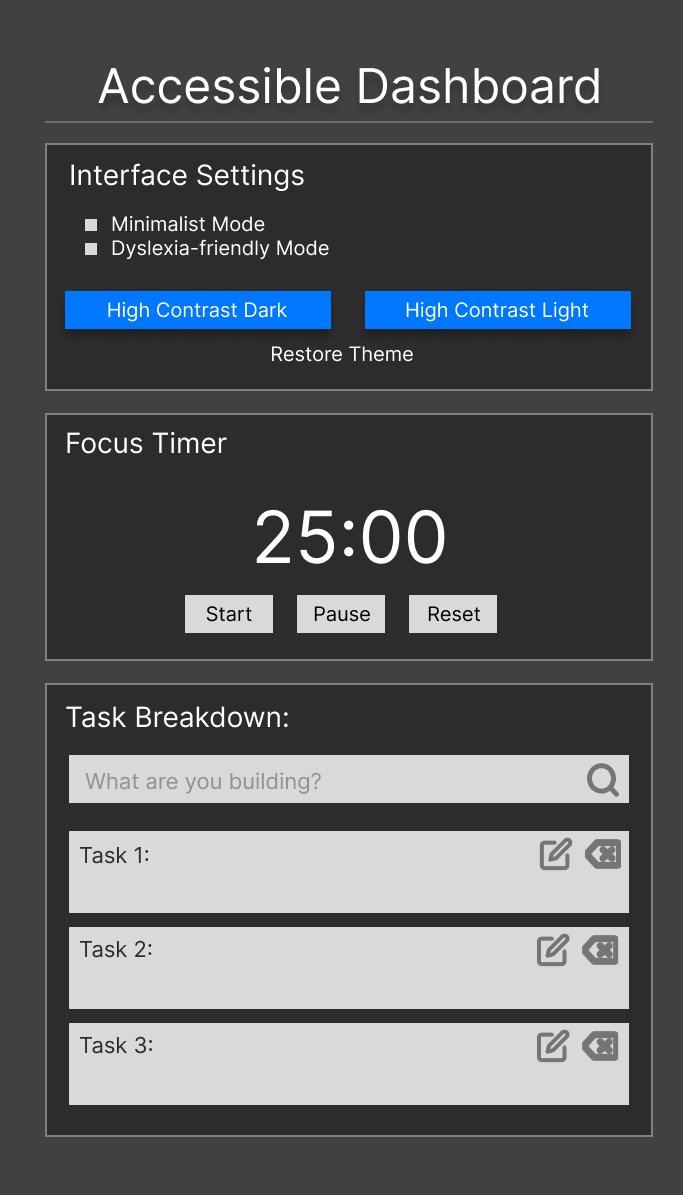
\includegraphics[width=0.6\linewidth, alt={}] {logos/Plug-in plan.png}
    \caption{UI Plan For the Accessible \gls{IDE} Plugin.}\label{fig:plug-inplan}
\end{figure}

THe first draft if the \gls{UI} was designed in figma, which allowed me get a clear vision of how the plugin would look and function. 
This also guaranteed that the design of the plugin was in line with the requirements that had been set out in the previous section.
Before having an a visual idea for the UI the plan was to implement it using HTML and CSS in a Webview, which allowed me to create a custom dashboard 
that could be easily accessed from within VS Code.

\subsection{Technology Stack}
The development of the plugin utilises a modern web-based stack compatible with the VS Code extension ecosystem to ensure high performance and seamless \gls{API} integration.
\begin{itemize}
    \item JavaScript: The primary programming language used for both the extension backend and the Webview frontend. It was chosen for its native compatibility with Node.js and its ability to handle asynchronous message passing between the UI and the extension host.
    \item Node.js: Acts as the runtime environment for the extension, providing the necessary \gls{API}s for file system access, process management, and the execution of imperative commands within the \gls{IDE}.
    \item VS Code Extension \gls{API}: The core framework used to manipulate the \gls{IDE} environment. Specifically, it facilitates interaction with workspace.getConfiguration for visual styling and vscode.commands for interface simplification.
    \item OpenAI \gls{API} / VS Code Language Model \gls{API}: Provides the generative intelligence required for the Task Architect and Code Explainer. By utilising the resident gpt-4o model, the plugin performs complex Chain of Thought~(\gls{CoT}) reasoning without requiring the user to provide personal \gls{API} keys.
    \item HTML/CSS: Used within the Webview layer to construct the Accessible Dashboard. This allows for the implementation of custom high-contrast themes and dynamic scaling that exceeds the limitations of standard VS Code CSS.
\end{itemize}

In terms of plugin development, the two main languages that are used
 are JavaScript and TypeScript. Although Typescript is more useful if the project was larger, I felt that JavaScript would be sufficient for the scope of this project and would 
 allow me develop the plugin quickly, especially due to the fast turn around time of the project. JavaScript was also chosen for its native compatibility with the VS Code 
 extension host and its ability to handle asynchronous message passing between the UI and backend.~\cite{TypeScri5:online}
 
For the \gls{AI} features, I decided to use the \textit{gpt-4o} model through the VS Code Language Model \gls{API}, which allows me to leverage powerful language models without 
requiring users to manage their own \gls{API} keys. Finally, I chose HTML and CSS for the Webview UI to allow for maximum flexibility in designing the dashboard 
and implementing custom themes. 

\subsubsection{Minimalist Toggle (FR1)}

The Minimalist Toggle serves as a reset for the \gls{IDE}. It utilises a state-management system to track the current visibility of the VS Code workbench.
When activated, it dispatches a batch of imperative commands to the vscode.commands \gls{API}, hiding the Activity Bar, Status Bar, Side Bar, and Breadcrumbs simultaneously.
By reducing the total number of visual elements on the screen, the module lowers extraneous cognitive load, allowing the developer to allocate more mental energy to the
code editor itself.


\subsubsection{Task Architect - \gls{AI}-Driven \Gls{scaffolding} (FR2)}
The Task Architect is a Human-in-the-Loop~(\gls{HITL}) module that facilitates \gls{task_initiation} by breaking down overwhelming objectives into granular steps. The module should employs 
a \gls{CoT} prompting strategy to take a complex task and break it down into simpler sub-tasks.
The generated steps are rendered as editable fields within the dashboard, allowing users to modify or refine the \gls{AI}'s suggestions. This ensures that developers 
maintain agency over their project architecture while the \gls{AI} handles the initial decomposition.
\newline

\textbf{Overcoming Latency and Verbosity}
\newline
During the testing of various prompt structures, a recurring challenge emerged, how much unnecessary text was included in the \gls{LLM}'s output.
 When asked to assist, the model frequently included excessive supportive dialogue. While intended to be user-friendly, this extra text hindered the system's 
 ability to parse the output into discrete, editable UI components.

To solve this issue, the prompt was refined to enforce a strict structural output, prioritising data over dialogue. This ensured that the generated steps 
could be seamlessly rendered as editable fields within the dashboard, preserving the developer's agency to modify or refine the architecture without sifting 
through conversational filler.


\textbf{Balancing Granularity and Utility}
\newline
Initial experiments with simple prompts such as ``How to code a login page'', the \gls{LLM} would bypass the architectural phase and provide a block of code immediately. 
This was counterproductive for two reasons:

\begin{itemize}
    \item It failed to provide a conceptual roadmap for the user.
    \item It increased the technical hallucination risk by attempting to solve a high-level task in a single step rather than planning the logic first.
\end{itemize}

\textbf{Increased Steps}
\newline
The original design specifications for the Task Architect called for 3 to 5 broad sub-tasks. However, user testing revealed that this flat structure remained overwhelming. A single step like ``Set up the backend'' was still too abstract for many users to execute confidently.
To address this, I implemented a hierarchical decomposition strategy. The system is now instructed to generate a primary set of sub-tasks, but with a critical addition: each sub-task must include two distinct micro-steps.

\subsubsection{Visual Styler} 
The Visual Styler is a specialised UI/UX module designed to manage the \gls{IDE}`s aesthetic environment, specifically targeting the reduction of eye strain and sensory overwhelm. By prioritising visual ergonomics, the module ensures that the development environment remains inclusive for \gls{neurodivergent} users and those with visual impairments.

\textbf{Accessibility and \gls{WCAG} Mapping}
\newline
To ensure the platform is accessible to the widest possible audience, the Visual Styler utilises a systematic mapping of presets based on the Web Content Accessibility Guidelines (WCAG) 2.1 Level AA.
\begin{itemize}
    \item High Contrast Modes: The module provides dedicated \textit{High Contrast Dark} and \textit{High Contrast Light} themes. These presets are programmatically validated to ensure a minimum contrast ratio of 4.5:1 for standard text and 3:1 for large text or UI components.
    \item Sensitivity Accommodations: By offering these specific color profiles, the \gls{IDE} addresses the needs of users with color vision deficiencies~(\gls{CVD}) and photophobia 
    (light sensitivity), allowing for a high-degree of legibility without triggering sensory fatigue.
\end{itemize}

\textbf{Technical Implementation and Functionality}
\newline
The Visual Styler operates by interacting directly with the workspace.getConfiguration \gls{API}. This allows the module to move beyond surface-level CSS changes and manipulate the core structural rendering of the workspace:

Dynamic Scaling: Users can adjust font sizes and line heights across the entire interface. Increasing the line height (e.g., to 1.5 or 2.0) is a critical intervention for developers with \gls{dyslexia}, as it reduces the crowding effect of text and improves character recognition.

Granular Customisation: Unlike traditional static themes, the Styler follows a visual comfort framework. It treats font-weight, letter spacing, and padding as variables that the user can tune to their specific cognitive load requirements.

User Agency and Sensory Regulation
By providing an intuitive dashboard for these adjustments, the Visual Styler empowers the developer to curate their own sensory environment. This reduces the cognitive energy spent on deciphering a cluttered or poorly-lit UI, allowing that energy to be redirected toward the primary task of programming. The module essentially acts as a sensory filter, ensuring that the \gls{IDE} adapts to the user`s biological needs rather than forcing the user to adapt to a rigid interface.

\subsection{System Architecture}
The system is divided into three primary layers: the Presentation Layer (Webview), the Orchestration Layer (Extension Host), and the External Services Layer (VS Code \gls{API}).

1. The Presentation Layer: WebView UI

The user interface is implemented as a \texttt{WebviewPanel}, which renders a custom HTML/JavaScript dashboard. This allows for a highly flexible UI where the extension to be customised to best fit the user's needs, predetermined through prior research.

\begin{itemize}
    \item State Communication: Because WebViews are isolated from the main editor, communication is handled via asynchronous message passing. The UI dispatches JSON-formatted messages using \texttt{vscode.postMessage()}, which are then intercepted by the extension’s backend.
    \item Asynchronous Feedback: The UI remains responsive by using event listeners that wait for \texttt{updateTime}, \texttt{taskResult}, or \texttt{errorResult} commands sent back from the extension host.
\end{itemize}

2. The Orchestration Layer: Extension Host

The core logic resides in the activate function, which serves as the central hub while the extension is active.

\begin{itemize}
    \item Command Registration: The system registers specific URI commands (e.g., accessible-toggle.showUI) that map user intents to internal JavaScript functions.
    \item Configuration Management: A key architectural feature is the interaction with getConfiguration. The extension reads and writes global settings to modify the editor's environment (font size, themes, and layout) in real-time, effectively acting as a wrapper for the VS Code Settings engine. 
    \item Context Preservation: To ensure the system is non-destructive, the architecture utilises \texttt{context.globalState}. This allows the extension to store the user`s original theme and font settings before applying accessibility modifications, enabling a seamless restoration process. This also acts as a form of error prevention in case any settings are applied by accident.
\end{itemize}


3. The Functional Providers

The architecture employs specialised logic blocks to handle distinct accessibility needs:

\begin{table}[ht]
    \centering
    \caption{System Component Interaction and \gls{API} Dependencies}\label{tab:system_architecture}
    \small % Slightly smaller text to ensure it fits the margins
    \begin{tabular}{@{} l p{4cm} l @{}}
        \toprule
        \textbf{Component} & \textbf{Interaction Strategy} & \textbf{VS Code API Dependency} \\ 
        \midrule
        Interface Controller & Imperative Commands          & \texttt{commands.executeCommand} \\
        Theme/Font Engine    & Configuration Updates        & \texttt{workspace.getConfiguration} \\
        Task Architect       & \gls{AI} Stream Processing         & \texttt{vscode.lm} (Language Model) \\
        Code Helper          & Diagnostic Polling           & \texttt{languages.getDiagnostics} \\
        \bottomrule
    \end{tabular}
\end{table}

4. Integration with Language Models 

The \textit{Task Architect} and \textit{Code Helper} features utilise the VS Code Language Model \gls{API}. This architectural choice ensures security and efficiency, as the extension does not require individual \gls{API} keys from the user. Instead, it requests access to the editor's resident models (e.g., GPT-4o). The system uses a \gls{CoT} prompting strategy to process raw diagnostic data or user goals into structured, \gls{neurodiverse}-friendly steps before pushing the data back to the Presentation Layer.


\subsection{UI Simplification and Minimalist Toggle (FR1)}
The implementation of the Minimalist Mode focuses on reducing visual noise, which research identifies as a primary driver of cognitive overload and sensory overwhelm for autistic and \gls{ADHD} developers.
 This module acts as a digital ramp, filtering environmental noise to prevent the exhaustion of a developer's limited cognitive budget.
 
 The technical execution follows an imperative command pattern to provide a seamless, one-click transition:
\begin{itemize}
 \item \textbf{Workspace Manipulation:} Using the vscode.commands.executeCommand \gls{API}, the plugin simultaneously toggles the visibility of the Activity Bar, Side Bar, Status Bar, and Breadcrumbs.
 \item \textbf{Global Configuration:} To remove persistent distractions like the Mini-map, the system interacts directly with global user settings using config.update('editor.minimap.enabled', ...).
 \item \textbf{State Management:} The module utilises a state-management system to track the current visibility of the VS Code workbench.
 \item \textbf{Non-Destructive Restoration:} To mitigate anxiety regarding lost settings, the architecture employs context.globalState to store the original UI configuration. This allows users to revert all changes instantly, satisfying the requirement for a safe and reversible interface.
 \end{itemize}

 By centralising these actions into a single toggle, the plugin lowers Extraneous Cognitive Load (\gls{EL}). This allows the developer to reallocate mental resources from navigating a complex, high-density interface toward \gls{GL}, the actual logical problem-solving and programming tasks

\textbf{Final UI/Functionality Integration (FR1)}
\begin{figure}[H]
    \centering
    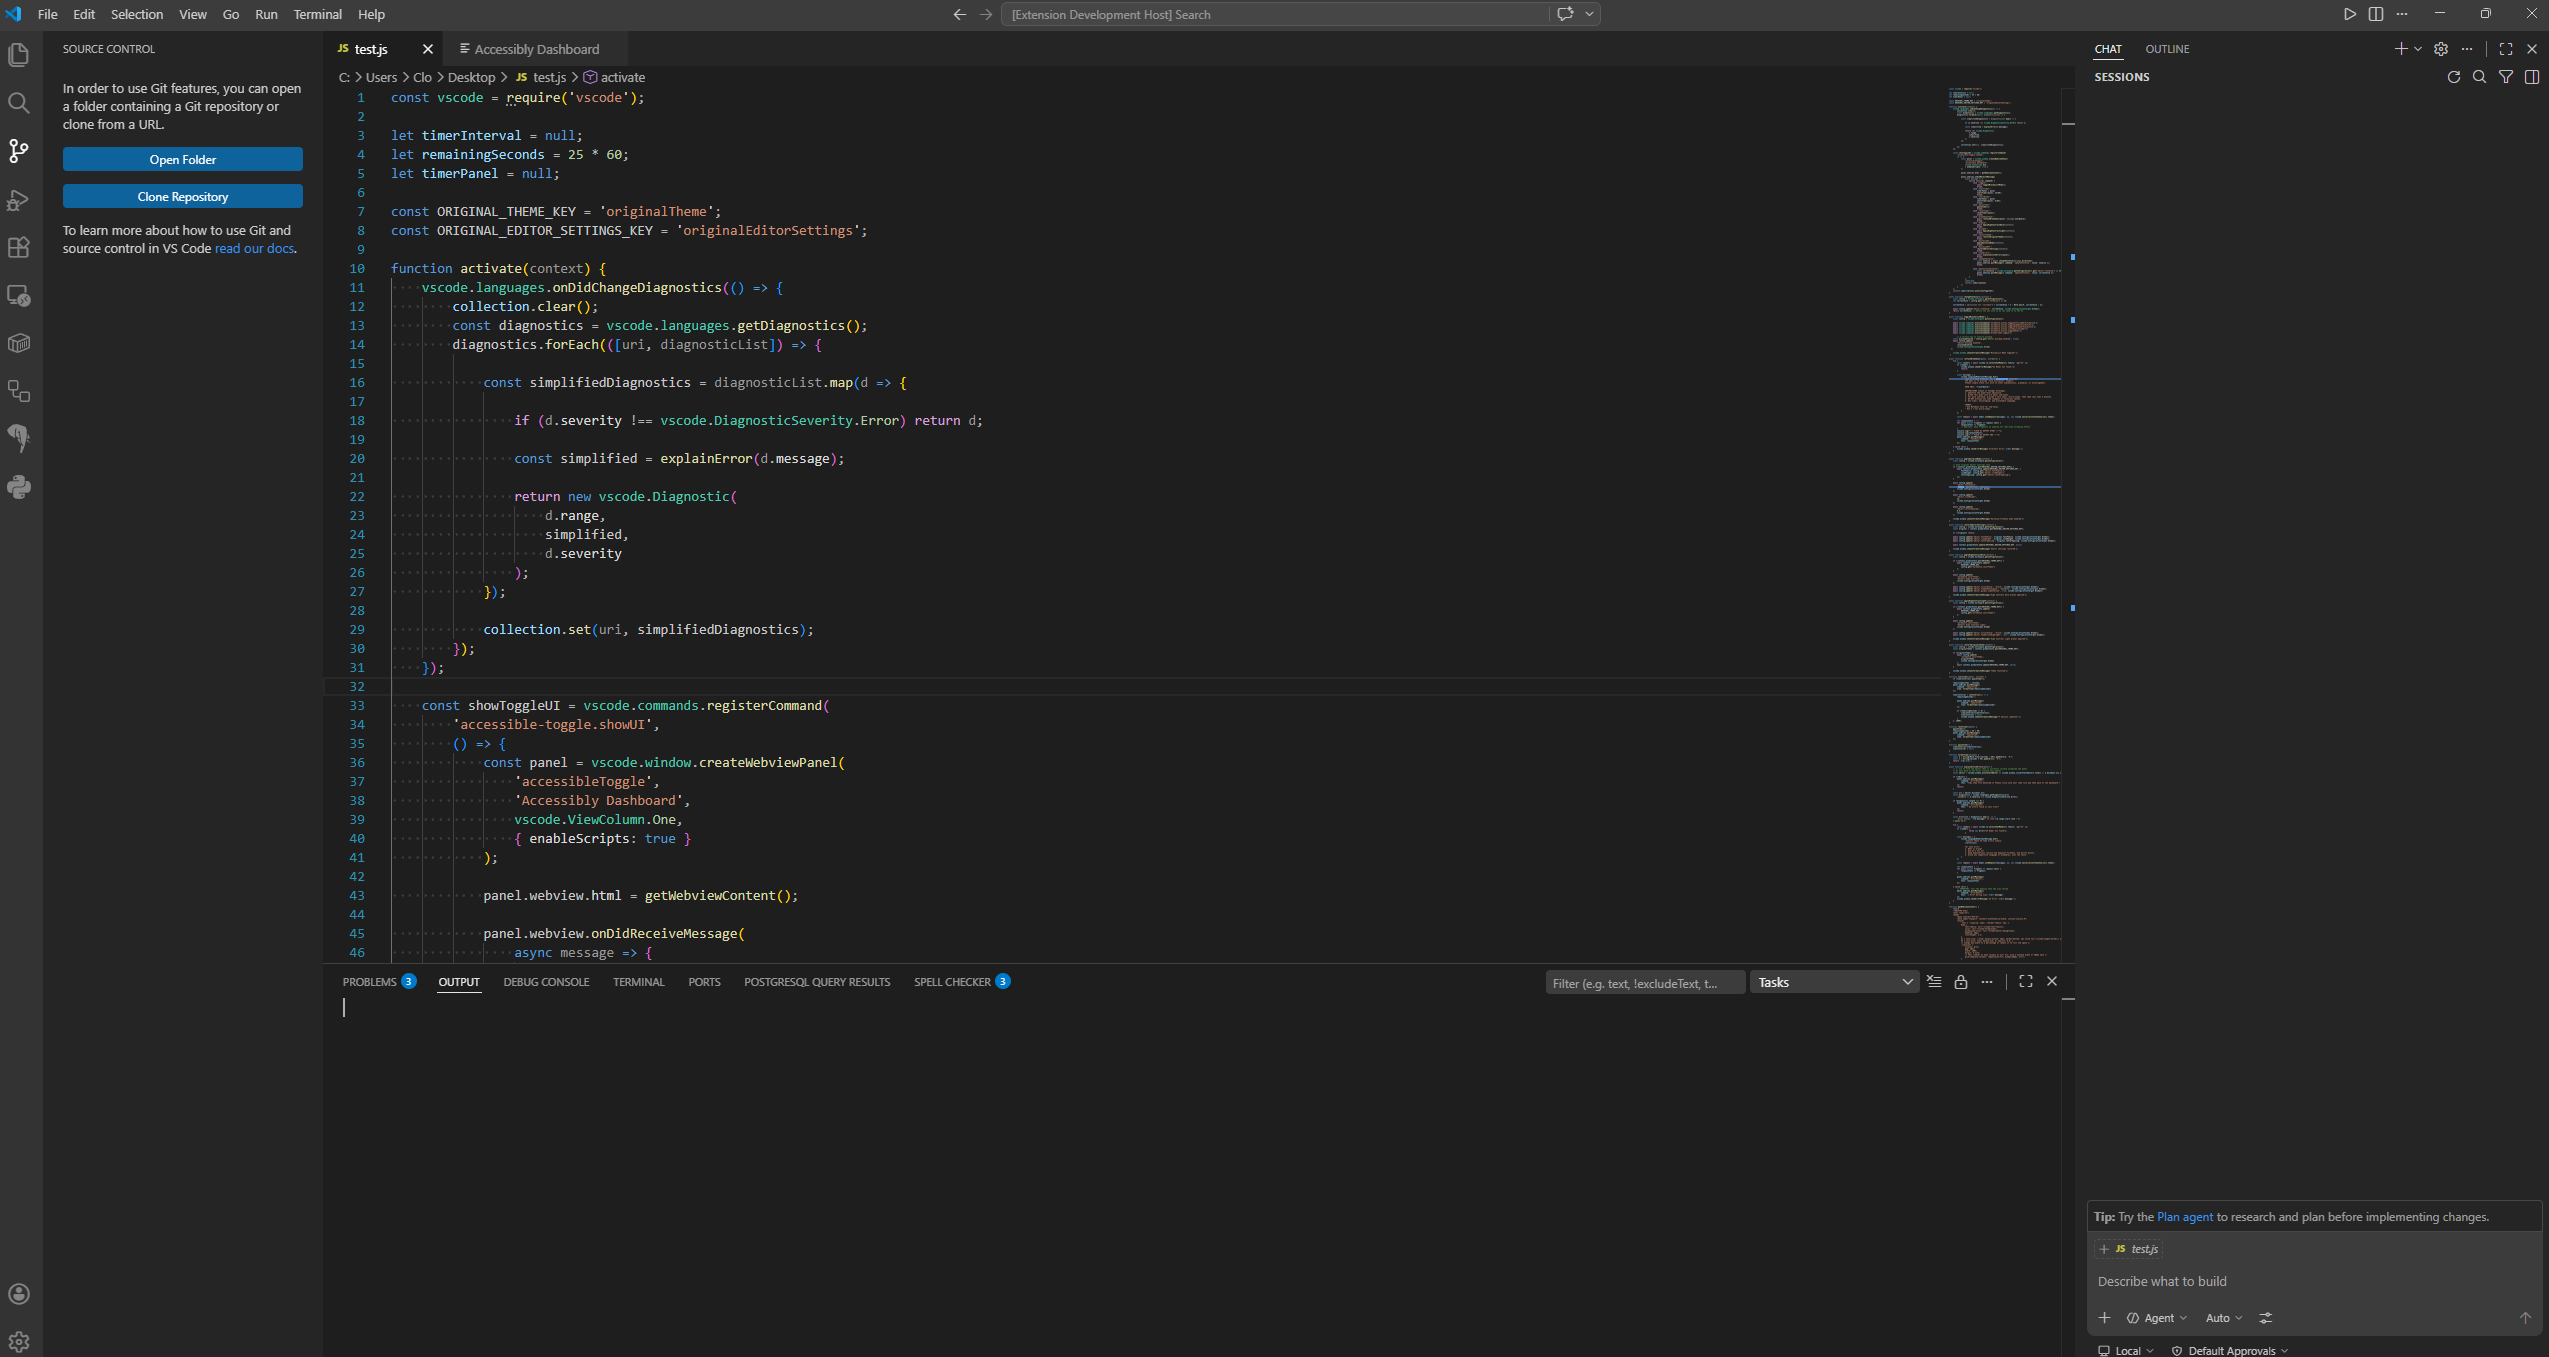
\includegraphics[width=0.9\linewidth, alt={}] {logos/preMinimal.png}
    \caption{Pre-Minimalist UI, showing the default VS Code interface with all standard elements visible.}\label{fig:PreMinimal}
\end{figure}

\begin{figure}[H]
    \centering
    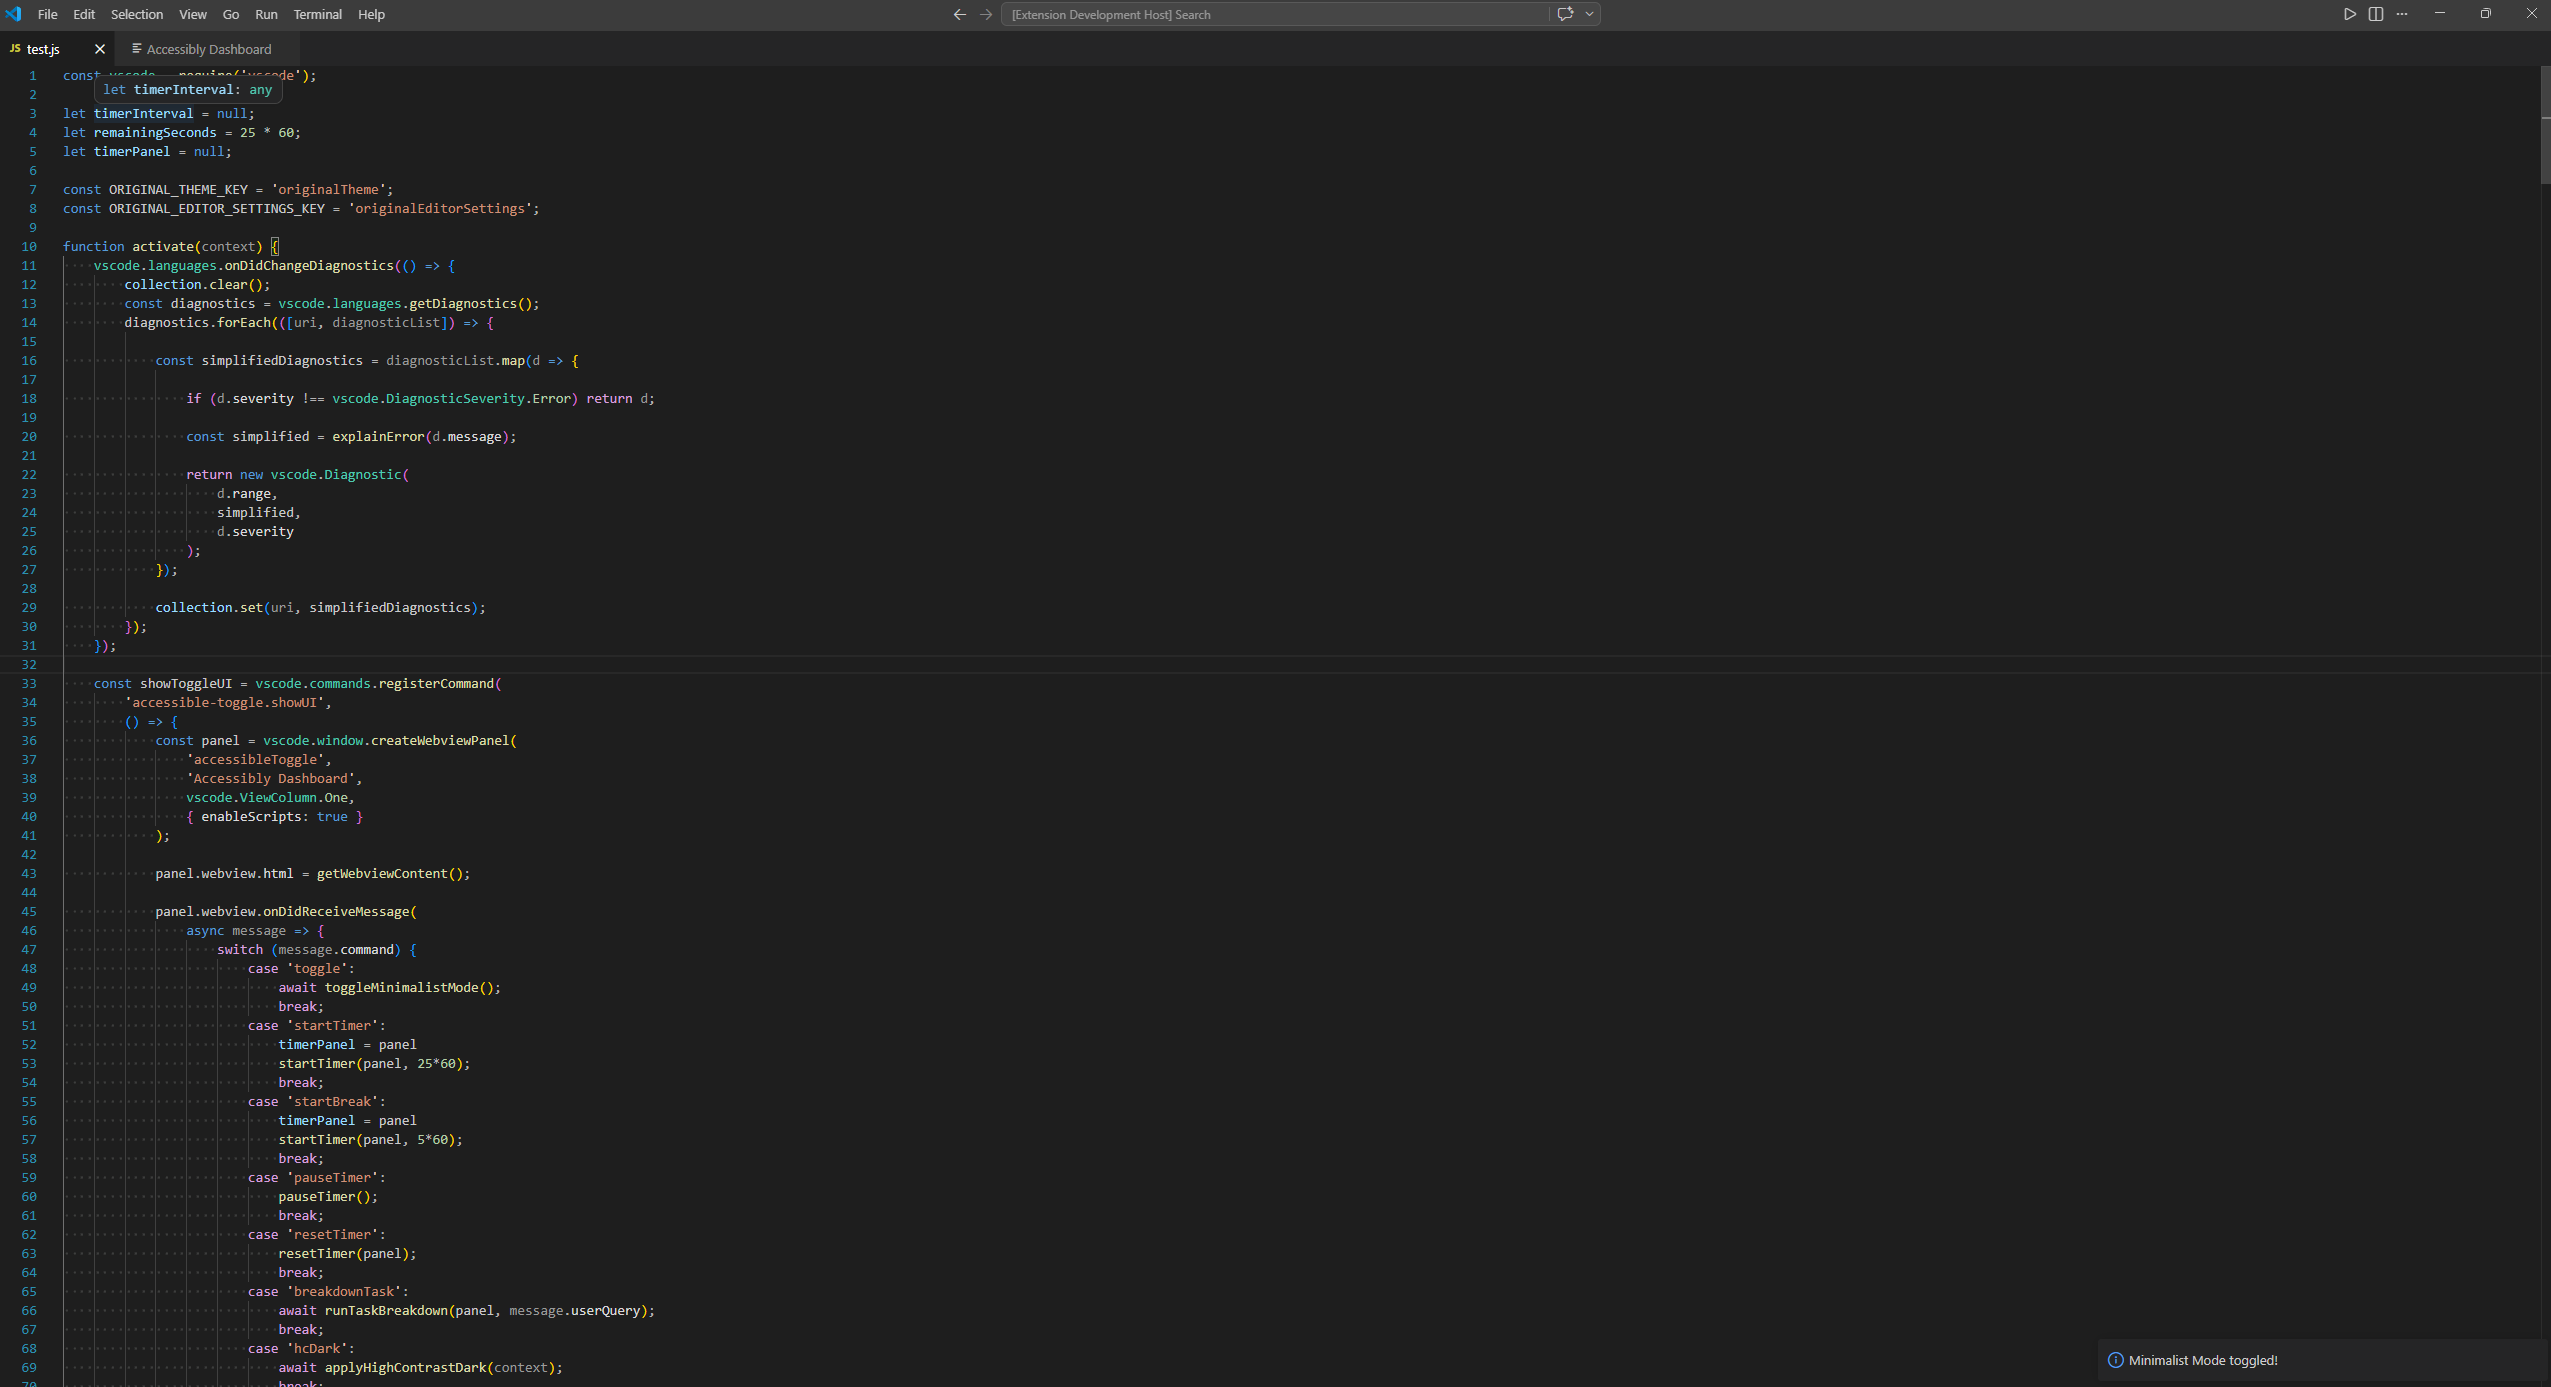
\includegraphics[width=0.9\linewidth, alt={}] {logos/postMinimal.png}
    \caption{Post-Minimalist UI, showing the simplified VS Code interface with reduced visual elements.}\label{fig:PostMinimal}
\end{figure}

\begin{figure}[H]
    \centering
    
\includegraphics[width=0.7\linewidth, alt={}] {logos/MinimalNote.png}
    \caption{Notification confirming the activation of Minimalist Mode, providing immediate feedback to the user.}\label{fig:MinimalNote}
\end{figure}

\subsection{\gls{AI} Integration (FR2 and FR3)}
The \gls{AI}-driven features are implemented using a Streaming Data Pattern to satisfy NFR3 (Latency), ensuring the interface remains responsive during complex generation.

\subsubsection{Task Architect: Overcoming \Gls{task_paralysis}}
\begin{itemize}
\item \textbf{Prompt Engineering:} The \textit{Task Architect} uses a strictly defined system prompt to enforce a micro-step structure (3--5 sub-tasks with two 5-minute 
micro-steps each). This prevents the \gls{LLM} from generating a long response that can be overwhelming.
\item \textbf{Iterative Prompt Refinement:} During development, I identified a significant limitation where the \gls{LLM} included excessive supportive dialogue 
(e.g., ``Sure! I can help with that''). While polite, this violated the principle of Direct Instruction and hindered the system's ability to parse the text into 
editable UI components. I refined the prompt to mandate a strict data-only format, ensuring the system only outputs actionable tasks.
\end{itemize}

\begin{figure}[H]
    \centering
    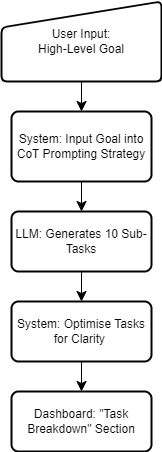
\includegraphics[width=0.3\linewidth, alt={}] {logos/aiflow.png}
    \caption{\gls{AI} Flow for the Task Architect Module.}\label{fig:AIflow}
\end{figure}

The Figure~\ref{fig:AIflow} demonstrates the process of the Task Architect module. When a user enters a high-level goal (e.g., ``Implement a search bar''), the system 
instructs the \gls{LLM} to output 3-5 actionable sub-tasks with 2 additional tasks from each of the sub-tasks.
 
\begin{figure}[H]
    \centering
    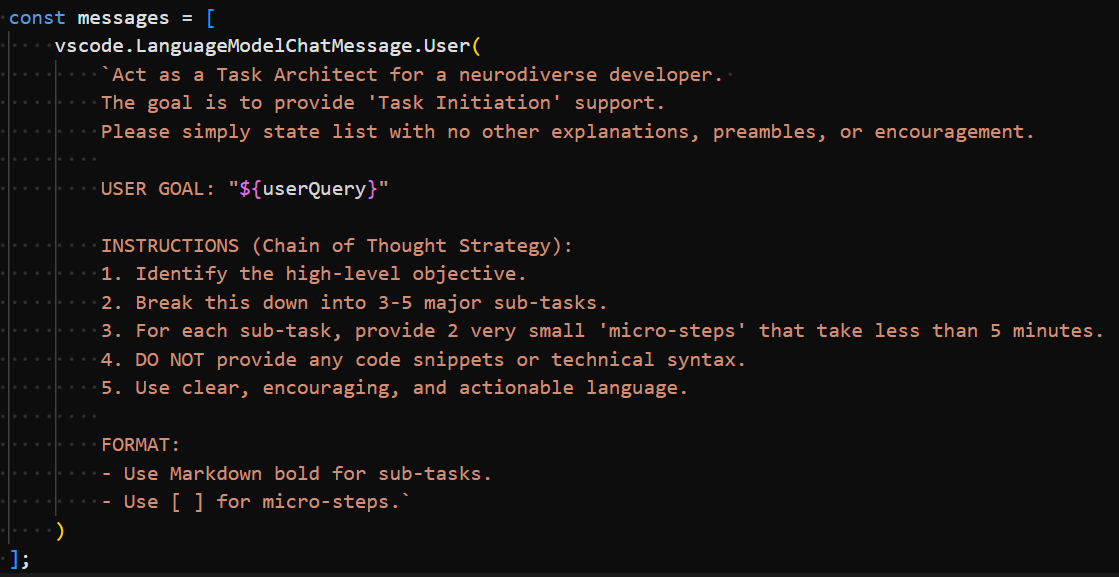
\includegraphics[width=1\linewidth, alt={}] {logos/aicode.png}
    \caption{Code written to generate tasks}\label{fig:AIcode}
\end{figure}

Not only does the this prompt ask the \gls{LLM} to break down the task, but it also instructs it to format the output in a specific way.
So that the response can be easily broken down and cleaned for the output the prompt includes instructions to make sure the subtasks in bold and the micro-steps are preceded by ``[ ]''.

\subsubsection{Human-in-the-Loop (HITL) Implementation}
As shown in Figures~\ref{fig:taskoutput} and~\ref{fig:taskarchitect}, the generated tasks are rendered in the dashboard as editable fields. This is a critical design choice to preserve User Agency. 
\Gls{neurodivergent} developers often have unique workflows so by allowing the user to edit or delete \gls{AI}-generated steps, the tool moves from being a prescriptive authority 
to a flexible partner. The graying-out of completed tasks provides immediate visual feedback, supporting \gls{working_memory} by externalising task progress.

\begin{figure}[H]
    \centering
    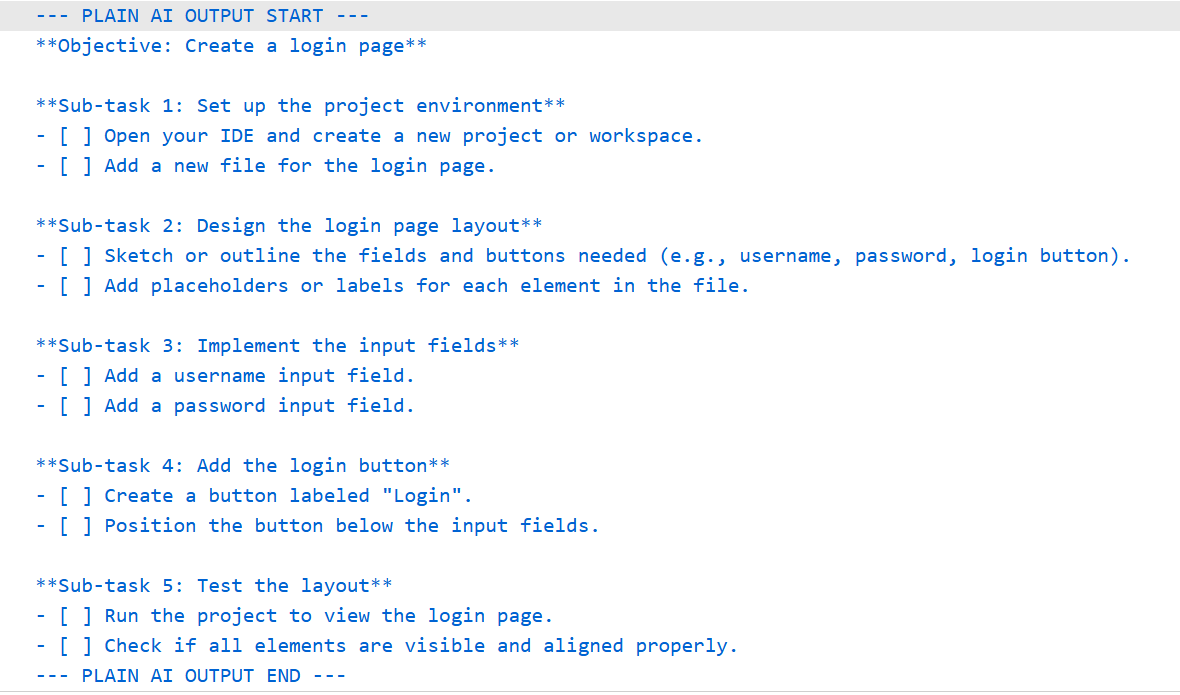
\includegraphics[width=0.8\linewidth, alt={}] {logos/taskoutput.png}
    \caption{Example of the output generated by the Task Architect module, showing the micro-steps for a given task.}\label{fig:taskoutput}
\end{figure}

\begin{figure}[H]
    \centering
    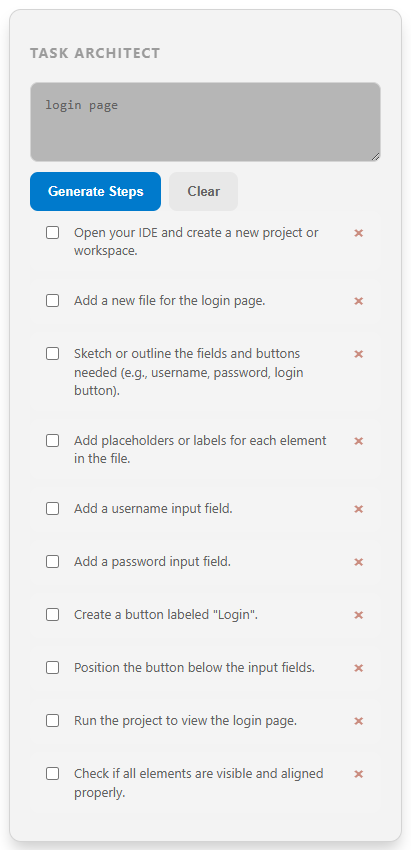
\includegraphics[width=0.6\linewidth, alt={}] {logos/taskarchitect.png}
    \caption{Task Architect Module in the Dashboard, showing the generated tasks.}\label{fig:taskarchitect}
\end{figure}

\subsubsection{Code Explainer: Mitigating Technical Cognitive Overload}
The Code Explainer is a diagnostic interceptor designed to address the high extraneous cognitive load often imposed by cryptic compiler errors. 
For neurodivergent developers, particularly those with \gls{ASD}, standard diagnostic messages can be ambiguous, leading to a breakdown in task 
momentum.

\textbf{Technical Implementation and Workflow}


The module is implemented as an asynchronous function, explainActiveErrors, which operates through a three-stage pipeline: Detection, Extraction, and Translation.
\begin{itemize}
    \item Detection: The system first verifies that a code file is active within the editor. If no file is detected, the system provides a clear, actionable 
instruction to the user: "No code file detected. Please click into your code file and then back to the dashboard." This ensures that the user understands 
the necessary context for the feature to function, reducing confusion and promoting a sense of control.
    \item Extraction: Using the vscode.languages.getDiagnostics \gls{API}, the module identifies active compiler issues. To minimise noise, 
    the system specifically filters for vscode.DiagnosticSeverity.Error, ensuring the developer is not overwhelmed by warnings or information-level 
    messages that do not immediately block execution.
    \item Translation: The raw error messages and their corresponding line numbers are compiled into an errorList string. 
This list is then dispatched to the resident \textit{gpt-4o} model via the VS Code Language Model \gls{API}.
\end{itemize}

\textbf{Prompt Engineering for Direct Instruction}


To satisfy the requirement for beginner-friendly, non-technical feedback, the module employs a strictly constrained system prompt. The \gls{AI} is instructed to:
\begin{itemize}
    \item Identify the problem and provide a specific fix.
    \item Maintain a concise, bulleted format.
    \item Avoid all \textit{supportive language} or conversational preambles.
\end{itemize}

This approach aligns with the principle of Direct Instruction, reducing the \gls{cognitive_tax} required to 
filter through polite but unnecessary conversational filler.

\subsection{\Gls{dyslexia} Settings: Test spacing (FR5)}
The Visual Styler module allows users to adjust the spacing between characters and line height in the \gls{IDE}. This is particularly beneficial for developers with \gls{dyslexia}, as increasing letter spacing 
and vertical padding can significantly reduce the crowding effect in dense code, improving character recognition and overall readability. 

    To balance customisability with cognitive ease, the plugin provides a set of predefined spacing presets, \textit{Standard, Relaxed, and Spacious},
for the users to choose from in the dashboard. This allows for quick adjustments without overwhelming the user with too many options, while still providing the 
necessary customisation to accommodate different cognitive needs.

The presets implement a hierarchical increase in visual breathing room:
\begin{itemize}
    \item Standard: Acts as a soft reset to default editor settings ($lineHeight: 0$, $letterSpacing: 0$) using the system's standard font family.
    \item Relaxed: Increases the $lineHeight$ to $30$ and $letterSpacing$ to $0.8$, introducing specialised fonts such as Lexend and OpenDyslexic.
    \item Spacious: Offers the maximum level of separation with a $lineHeight$ of $40$ and $letterSpacing$ of $1.5$. This preset prioritises OpenDyslexic as the primary font to further enhance character distinction.
\end{itemize}

The inclusion of OpenDyslexic and Lexend is a critical design choice; these fonts use 
weighted bottoms or unique shapes to help the brain distinguish between similar
characters (e.g., ``b'' vs ``d''), which is a common hurdle for dyslexic readers. 
By offering these as a unified \textit{Spacious} preset, the plugin provides a high-signal 
environment that accommodates diverse cognitive needs with minimal interaction cost.

\subsubsection{Initial Plan: One Option}
Initially, the plugin was programmed with fixed values for line height and letter spacing. 
However, user testing revealed that a one-size-fits-all approach was insufficient, as 
individual cognitive needs regarding text density vary significantly.

The figures below demonstrate the visual impact of these adjustments. 
Figure~\ref{fig:vanillasettings} displays the standard VS Code environment, 
while Figure~\ref{fig:dyslexiasettings} illustrates the enhanced readability achieved
 by increasing the line height to 1.5 and the letter spacing to 0.5em.

\begin{figure}[H]
    \centering
    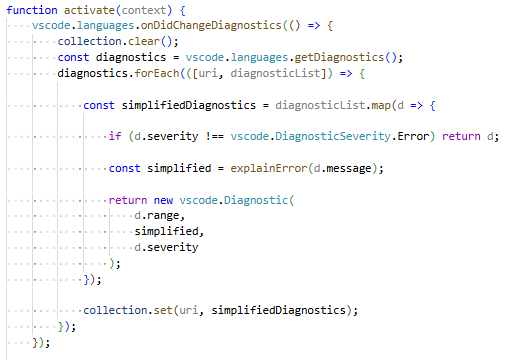
\includegraphics[width=0.7\linewidth, alt={}] {logos/van.png}
    \caption{Example of the difference in spacing between the default settings and the original \gls{dyslexia} settings, where the line height is set to 1.5 and the letter spacing is set to 0.5em.}\label{fig:vanillasettings}
\end{figure}

\begin{figure}[H]
    \centering
    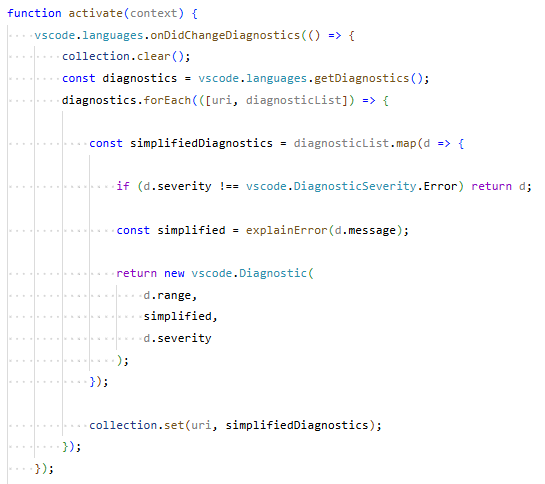
\includegraphics[width=0.7\linewidth, alt={}] {logos/bas.png}
    \caption{Example of the difference in spacing between the default settings and the original \gls{dyslexia} settings, where the line height is set to 1.5 and the letter spacing is set to 0.5em.}\label{fig:dyslexiasettings}
\end{figure}

\subsubsection{Final UI Integration}
The final UI design (see Figure~\ref{fig:dyslexiamenu}) unifies the Visual Styler with other cognitive aids to ensure that environment modification is non-destructive and instantaneous:
\begin{figure}[H]
    \centering
    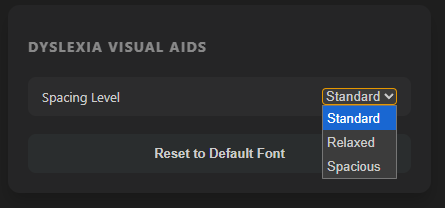
\includegraphics[width=0.7\linewidth, alt={}] {logos/dislecMenu.png}
    \caption{The UI implementation of the line spacing tool}\label{fig:dyslexiamenu}
\end{figure}
The evolution from fixed values to the hierarchical preset system (Standard, Relaxed, Spacious) 
represents a shift toward a user-centric sensory model. By centralising these 
complex font and spacing configurations into a single module within the 
Accessible Dashboard, the plugin minimises the executive tax required to curate
a readable workspace.

\begin{itemize}
    \item One-Click Presets: Instead of navigating nested VS Code menus, users select the \textit{Dyslexia-friendly Mode} or specific high-contrast buttons. This reduces interaction depth from approximately six clicks to one, significantly lowering extraneous cognitive load.
    \item Immediate Visual Confirmation: The dashboard provides real-time feedback, eliminating the verification anxiety common when \gls{neurodivergent} users must exit menus to see if changes were applied.
    \item Typography Hierarchy: The final implementation ensures that selecting a preset like \textit{Spacious} simultaneously updates three variables: increasing $lineHeight$ to 40, $letterSpacing$ to 1.5, and switching the typeface to OpenDyslexic.
    \item Non-Destructive Restoration: A critical component of the final UI is the \textit{Restore Theme} and reset functionality. This allows developers to experiment with spacing and contrast without the anxiety of losing their original, custom \gls{IDE} configurations.
\end{itemize}

\begin{figure}[H]
    \centering
    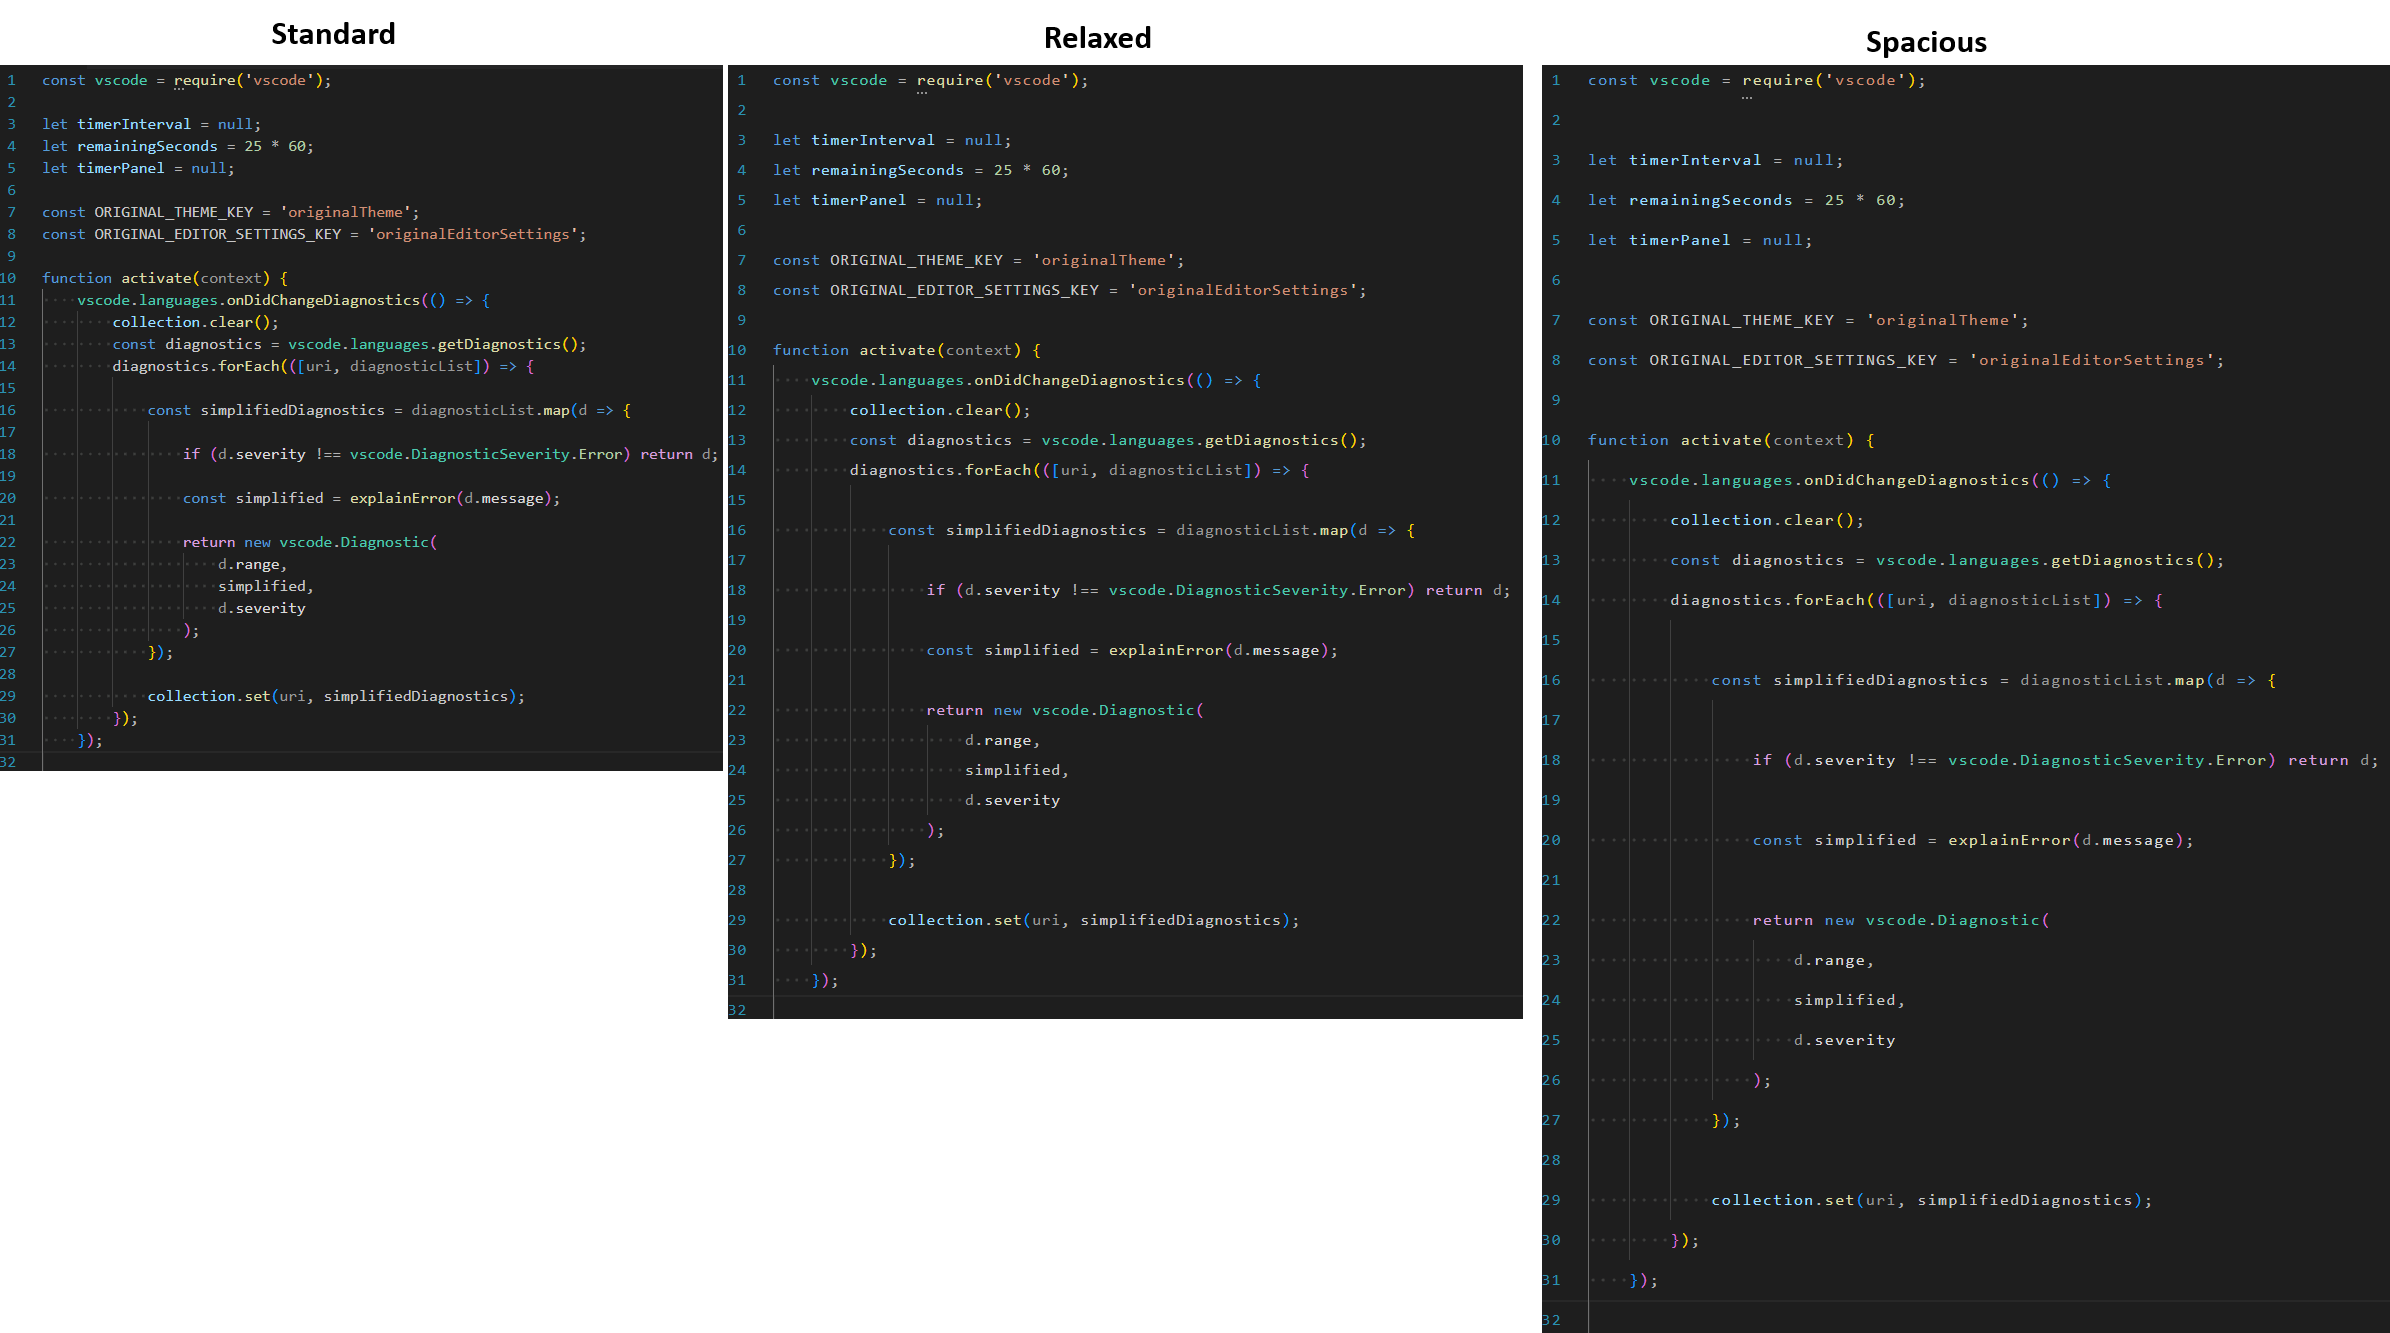
\includegraphics[width=1.6\linewidth, angle=90, alt={}] {logos/textOptions.png}
    \caption{Text spacing options implemented}\label{fig:dyslexiaText}
\end{figure}

\subsection{Pomodoro Timer (FR4)}
As mentioned in the literature review, the Pomodoro technique can be an effective tool for managing time and maintaining focus, especially for individuals with \gls{ADHD}. 
The plugin includes a customisable Pomodoro timer that allows users to set their own focus intervals and break durations. This flexibility is crucial, as a standard
 25-minute focus period may not be suitable for everyone.

The timer is integrated into the dashboard, providing a visual countdown and notifications when it's time to take a break or return to work. By allowing users to tailor 
the timing to their own rhythms, the plugin helps to reduce \glspl{state_recovery_cost} associated with interruptions and supports sustained focus.

\begin{figure}[H]
    \centering
    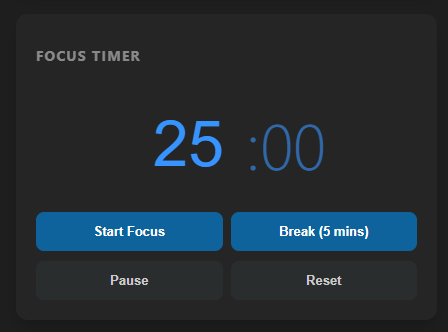
\includegraphics[width=0.6\linewidth, alt={}] {logos/timerFinal.png}
    \caption{Final design of the Pomodoro timer. The timer is directly editable, allowing users to set their own focus and break durations.}
    \label{fig:TimerFinal}
\end{figure}

\subsection{Initial User Testing and Feedback}
Initial user testing focused on the plugin's usability and functionality, revealing three critical areas for improvement. These are: 
UI clarity, \gls{AI} reliability, and efficiency. Feedback indicated that original labels like ``Decompose'' were too abstract, 
leading to a redesign of the Task Architect with clearer button labeling (``Generate Steps'') and contextual placeholders.
\begin{figure}[H]
    \centering
    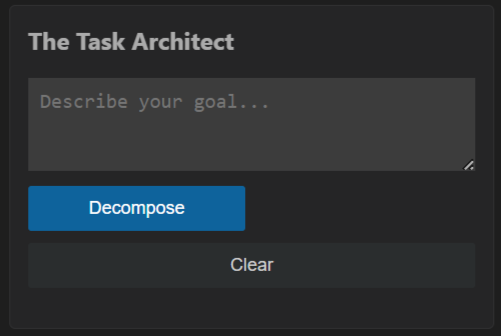
\includegraphics[width=0.6\linewidth, alt={}] {logos/uiprefix1.png}
    \caption{UI at the time of initial user testing, before improvements to the UI and \gls{AI} response integrity were made.}\label{fig:uiprefix}
\end{figure}

\begin{figure}[H]
    \centering
    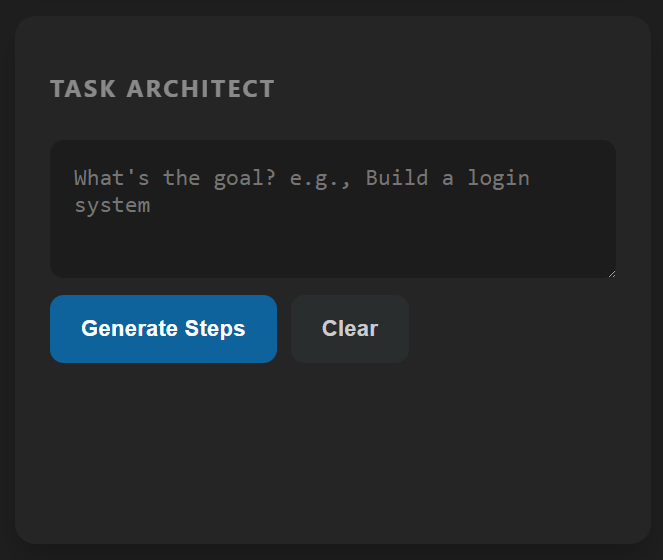
\includegraphics[width=0.6\linewidth, alt={}] {logos/uipostfix1.png}
    \caption{UI after improvements to the UI and \gls{AI} response integrity were made.}\label{fig:uipostfix}
\end{figure}


Technical evaluations also identified a parsing bug that truncated \gls{AI} responses, which was resolved by implementing a robust 
regular expression strategy to ensure full rendering of micro-steps. Finally, comparative testing against standard VS 
Code demonstrated the plugin's ability to significantly reduce cognitive load; specifically, the user performed accessibility 
adjustments,such as theme switching, in just 1.9 seconds (one click) compared to 19.9 seconds (six clicks) in the standard \gls{IDE}. 
These refinements ensured the tool successfully provided a more direct, inclusive path for \gls{task_initiation} and environment customisation.

\subsection{Final UI}
The final UI of the Accessibly Dashboard (see Figure~\ref{fig:finalui}) serves as the unified control center for the plugin`s assistive features. 
Designed as a centralised Webview panel, it provides a low-friction entry point that reduces the executive tax required to manage 
a complex development environment.

The interface is structured into modular sections to support inhibitory control and \gls{working_memory}:

\textbf{Interface Settings and Theme Presets}
\begin{itemize}
\item Minimalist Toggle: A single-click switch ("Close Panels") that simultaneously hides the Activity Bar, Side Bar, Status Bar, 
and Breadcrumbs to suppress Extraneous Cognitive Load.
\item Dyslexia Mode: A global toggle to quickly apply readability enhancements.
\item Soft High Contrast: Includes presets like "Soft HC Dark" and "Soft HC Light" to provide high signal without the sensory 
\gls{halation} risks of pure black-and-white themes.
\item Restore Original: A non-destructive reset button that supports psychological safety by allowing users to instantly 
revert all environmental changes.
\end{itemize}

\textbf{\Gls{dyslexia} Visual Aids and Text Scaling}
\begin{itemize}
\item Hierarchical Spacing: A dropdown menu offering Standard, Relaxed, and Spacious presets. Selecting \textit{Spacious} programmatically 
adjusts line height to 40, letter spacing to 1.5, and switches the font to OpenDyslexic.
\item Granular Scaling: A dedicated text scaling module allows users to tune the font size in real-time, providing immediate visual 
confirmation and eliminating verification anxiety.
\end{itemize}

\textbf{AI-Driven \Gls{scaffolding}}
\begin{itemize}
    \item Task Architect: A Human-in-the-Loop (HITL) module where users input high-level goals. The \gls{AI} decomposes these into structured, 
editable checklists, mitigating the \gls{task_paralysis} common in \gls{ADHD} and \gls{ASD} profiles
    \item Code Helper: A diagnostic interceptor that translates cryptic compiler errors into plain-language instructions, limited to 
three bullet points to prevent cognitive overload.
\end{itemize}

\textbf{Time Management}
\begin{itemize}
    \item Focus Timer: An integrated Pomodoro timer that allows for user-defined focus and break durations. This externalises time to 
support developers with \gls{time-blindness} and prevents burnout from unregulated \gls{hyperfocus}.
\end{itemize}

The transition to this final dashboard reduced the time required for accessibility adjustments from 19.9 seconds (six clicks) 
in a standard \gls{IDE} to just 1.9 seconds (one click), representing a significant improvement in operational efficiency.

\begin{figure}[H]
    \centering
    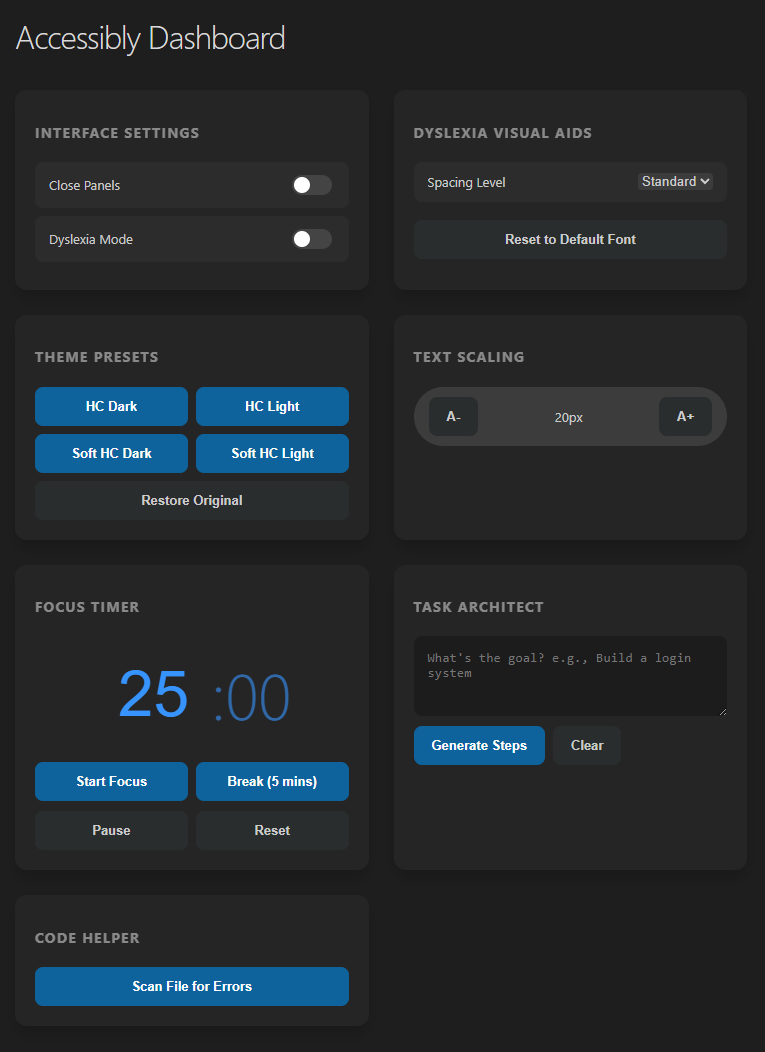
\includegraphics[width=1\linewidth, alt={}] {logos/Final.png}
    \caption{Final UI design.}\label{fig:finalui}
\end{figure}

\subsection{Evaluation and Methodology}

\subsubsection{Ethical Considerations}
Since this project involves human participants and also targets a vulnerable population, ethical considerations are 
paramount. The study will adhere to the following ethical guidelines:
\begin{itemize}
    \item \textbf{Informed Consent:} All participants will have the study fully explained to them, including the purpose, procedures. 
    \item \textbf{Confidentiality:} No names or personally identifiable information will be collected. Including information about the participants' neurodivergent status.
    \item \textbf{Voluntary Participation:} Participation in the study will be entirely voluntary, with no penalties for withdrawal at any stage.
\end{itemize}

\subsubsection{Experimental Design}
This study employs a \textit{within-subjects comparative design}, where each participant acts as their own control. This design is particularly effective for \gls{neurodivergent} research as it accounts for the high degree of individual variance in cognitive processing styles \cite{verma2025differences}. Participants will perform two standardised programming tasks: a project-planning phase and a debugging phase.

\begin{enumerate}
    \item \textbf{Control Condition:} Tasks are performed using a standard \gls{IDE} installation.
    \item \textbf{Experimental Condition:} Tasks are performed using the \gls{IDE} equipped with the Accessible Plugin features (Minimalist Toggle, Task Architect, and Visual Styler).
\end{enumerate}

To mitigate the \textit{carry-over effect} (where learning from the first task makes the second easier), the order of conditions will be counterbalanced, and task sets of equivalent \gls{IL} will be used across both conditions.

\subsubsection{Quantitative and Qualitative Frameworks}
To evaluate the efficacy of the plugin in reducing \gls{EL} and supporting \gls{executive_dysfunction}, two validated instruments will be administered.

\textbf{NASA Task Load Index (\gls{NASATLX})}


The \gls{NASATLX} is a multidimensional assessment tool used to quantify perceived workload. It is uniquely suited for this study as it allows for the isolation of specific cognitive pressures. While all six subscales will be measured to ensure a comprehensive view, the analysis will focus specifically on four key dimensions:

\begin{itemize}
    \item \textbf{Mental Demand:} To assess if the Task Architect successfully reduces the executive function tax required for project initiation.
    \item \textbf{Performance:} To measure the user's self-perception of success in the face of syntax errors or logic bugs.
    \item \textbf{Effort:} To quantify the total mental resources required to reach the goal.
    \item \textbf{Frustration:} Critical for \gls{neurodivergent} populations, this measures the emotional cost of switching between tasks and sensory overwhelm.
\end{itemize}

To evaluate the cognitive and physical demands of both interfaces, a NASA Task Load Index (\gls{NASATLX}) was administered to all participants ($N=5$).
I calculated both the Raw TLX ($r$-score) and the Weighted TLX ($w$-score) to account for individual differences in workload perception. 
The weighting factors were determined by the most important criteria, with Mental Demand (5) and Frustration (4) identified as the primary contributors to workload 
 in this task environment. Factors such as Temporal Demand and Physical Demand were weighted lower, reflecting their lesser impact on the overall workload in this context.

\begin{table}[h]
\centering
\caption{\gls{NASATLX} Weighting Factors}
\begin{tabular}{@{}p{1cm}p{1cm}p{1cm}p{1cm}p{1cm}p{1cm}@{}} % Fixed width for even spacing
\toprule
\textbf{MD} & \textbf{PD} & \textbf{TD} & \textbf{PF} & \textbf{EF} & \textbf{FR} \\ \midrule
5           & 1           & 0           & 3           & 2           & 4           \\ \bottomrule
\end{tabular}
\end{table}
\textbf{System Usability Scale (\gls{SUS})}


To assess the reliability and integration of the tool, the \gls{SUS} will be administered following the Experimental Condition. The \gls{SUS} is a 10-item questionnaire using a 5-point Likert scale, providing a global view of system usability. 

In the context of this study, the \gls{SUS} serves two primary purposes:
\begin{enumerate}
    \item \textbf{Integration Assessment:} Identifying if the \textit{Minimalist Toggle} feels like a seamless part of the workflow or an added complexity.
    \item \textbf{Confidence and Learnability:} Measuring the activation energy required to use the \gls{AI} features. For a developer experiencing \gls{task_paralysis}, a tool that is perceived as irritating to use (Item 8) or complex (Item 2) would be counter-productive.
\end{enumerate}

\subsubsection{Data Collection and Analysis}
In addition to the questionnaires, the study will record \textit{Time-on-Task} (to measure efficiency) and use a \textit{Think-Aloud Protocol}. This qualitative approach will capture real-time instances of \glspl{state_recovery_cost} following an interruption, providing insight into how the \gls{AI} \gls{scaffolding} supports the developer in regaining \gls{hyperfocus}.

\newpage
\section{Results and Discussion}

\subsection{NASA-TLX Subjective Workload}
As shown in Table~\ref{tab:nasa_tlx_results}, participants reported consistently lower weighted NASA-TLX scores when using the dashboard interface compared to the standard \gls{IDE}.
These reductions were most pronounced in Mental Demand, Effort, and Frustration, suggesting that the dashboard primarily reduces interface-driven 
extraneous cognitive load.
\begin{table}[H]
\centering
\caption{NASA-TLX Results for Standard vs Dashboard Interfaces}
\resizebox{\textwidth}{!}{%
\begin{tabular}{llccccccccc}
\hline
Participant & Interface & MD & PD & TD & PF & EF & FR & r-score & w-score \\
\hline
    1 & standard  & 60 & 10 & 0 & 30 & 50 & 60 & 35.0000 & 49.3333 \\
    1 & dashboard & 10 & 10 & 0 & 0  & 10 & 10 & 6.6667  & 8.0000  \\
    2 & standard  & 35 & 20 & 0 & 5  & 30 & 40 & 21.6667 & 28.6667 \\
    2 & dashboard & 5  & 10 & 0 & 0  & 10 & 15 & 6.6667  & 7.6667  \\
    3 & standard & 65 & 15 & 0 & 35 & 55 & 65 & 39.1667 & 54.3333 \\
    3 & dashboard & 15 & 5  & 0 & 5  & 10 & 15 & 8.3333  & 11.6667 \\
    4 & standard & 55 & 10 & 0 & 25 & 45 & 55 & 31.6667 & 44.6667 \\
    4 & dashboard & 10 & 5  & 0 & 5  & 10 & 5  & 5.8333  & 7.3333  \\
    5 & standard & 50 & 5  & 0 & 5  & 50 & 50 & 26.6667 & 38.0000 \\
    5 & dashboard & 5  & 5  & 0 & 0  & 5  & 5  & 3.3333  & 4.0000  \\
\hline
\end{tabular}%
}\label{tab:nasa_tlx_results}
\end{table}


\subsection{Workload Comparison and Interpretation}
The results indicate a substantial reduction in perceived workload when using the Dashboard interface compared to the standard interface.

\begin{itemize}
\item \textbf{Overall Workload:} The mean Weighted Score ($w$-score) for the standard interface was $43.00$ ($\sigma = 10.02$), which was reduced to $7.73$ ($\sigma = 2.72$) 
 with the Dashboard. This represents an approximate 82\% reduction in total perceived workload. 
\item \textbf{Cognitive Load:} The most dramatic improvement was observed in Mental Demand, which dropped from a mean of $53.0$ to $9.0$. This suggests that the Dashboard
 successfully offloaded information processing requirements from the user.
\item \textbf{Frustration and Effort:} Participants reported significantly lower levels of frustration ($10.0$ vs $54.0$) and required less effort ($9.0$ vs $46.0$) 
to complete the tasks using the Dashboard. 
\end{itemize}

\begin{figure}[H]
    \centering
    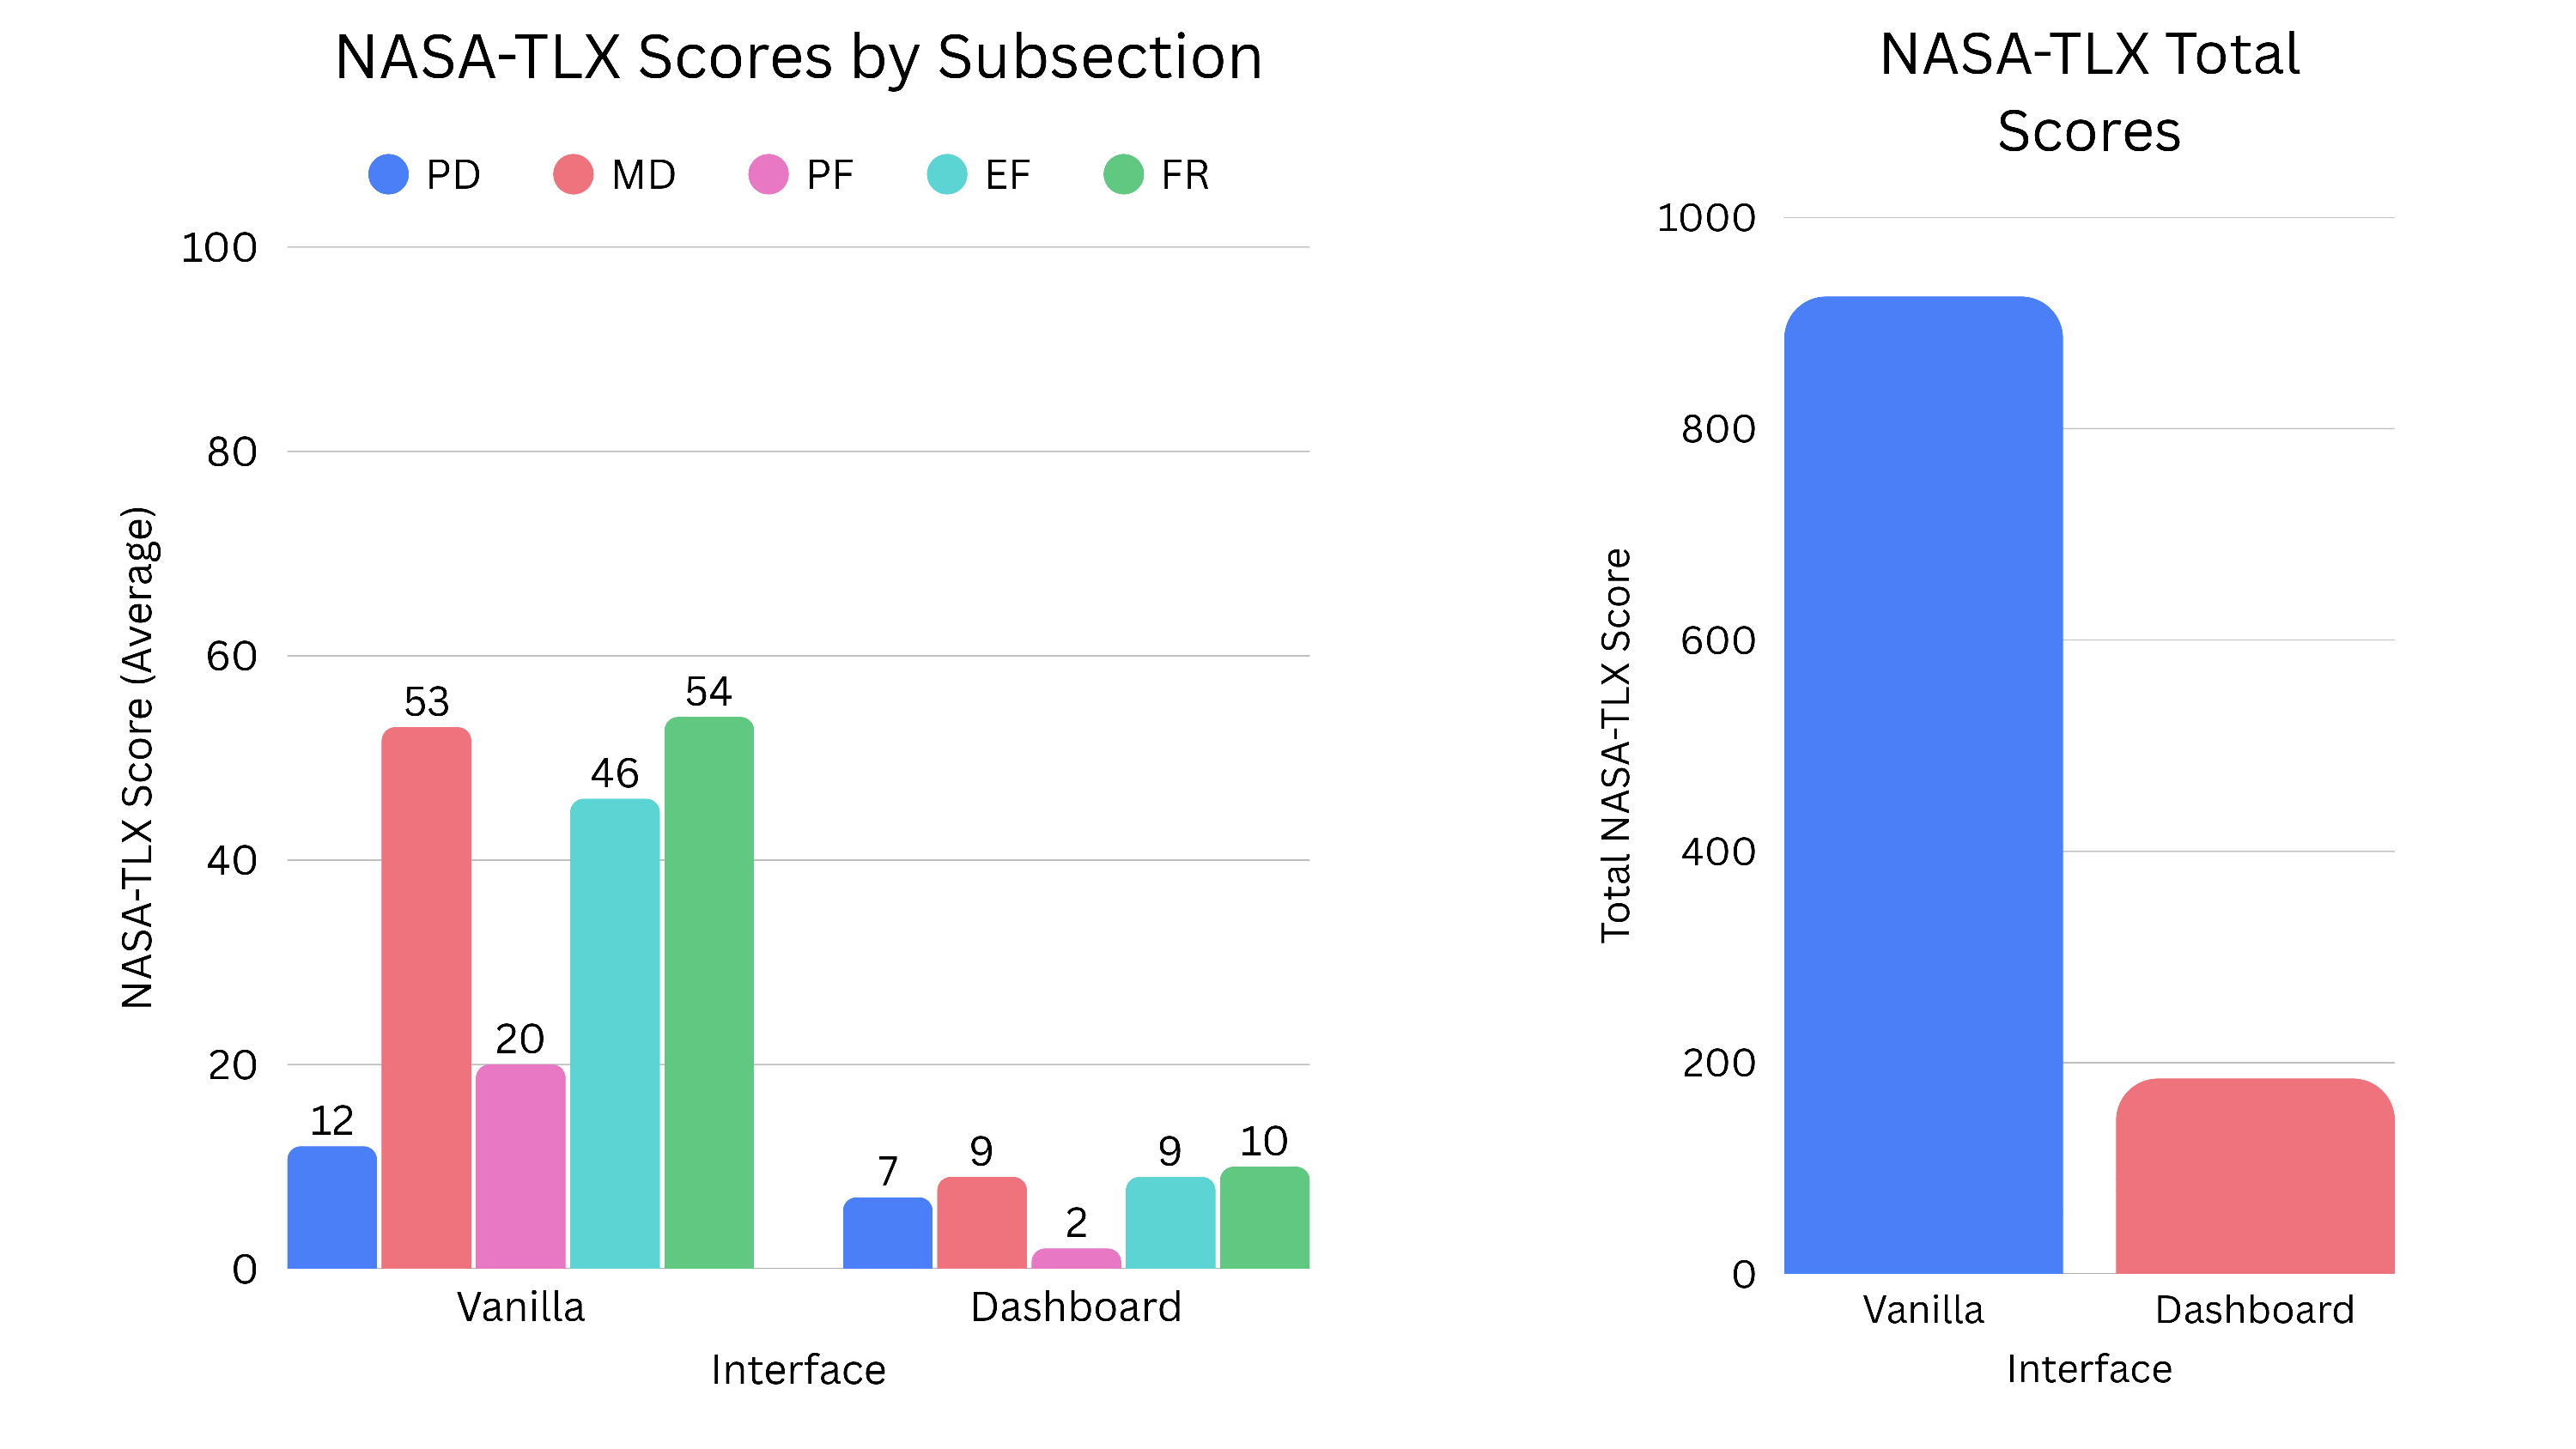
\includegraphics[width=1\textwidth]{Charts/nasatlxGraph.pdf} 
    \caption{Two graphs displaying the differences in the NASA-TLX scores for the two interfaces}\label{fig:Overallchart}
\end{figure}

These results suggest that the Dashboard's design effectively reduces the executive tax imposed by traditional \glspl{IDE}, allowing users to reallocate 
cognitive resources from interface navigation to core problem-solving. The significant reductions in Mental Demand and Frustration indicate that 
the Dashboard successfully mitigates key barriers to productivity for \gls{neurodivergent} developers, such as cognitive overload and interface-driven stress.

Even though the results are very positive, it is important to note that the small sample size ($N=5$) limits the generalisability of these findings. 
Future research with larger and more diverse participant pools is necessary to validate these results and ensure they apply across different populations of developers.


\begin{table}[h]
\centering
\caption{Summary of NASA-TLX Workload Scores (Mean $\pm$ SD)}
\label{tab:tlx_summary}
\begin{tabular}{lrr}
\toprule
\textbf{Workload Metric} & \textbf{Standard Interface} & \textbf{Dashboard Interface} \\
\midrule
Mental Demand    & 53.00 $\pm$ 11.51 & 9.00 $\pm$ 4.18  \\
Physical Demand  & 12.00 $\pm$ 5.70  & 7.00 $\pm$ 2.74  \\
Temporal Demand  & 0.00 $\pm$ 0.00   & 0.00 $\pm$ 0.00  \\
Performance* & 20.00 $\pm$ 14.14 & 2.00 $\pm$ 2.74  \\
Effort           & 46.00 $\pm$ 9.62  & 9.00 $\pm$ 2.24  \\
Frustration      & 54.00 $\pm$ 10.25 & 10.00 $\pm$ 5.00 \\
\midrule
\textbf{Weighted Score (Overall)} & \textbf{43.00 $\pm$ 9.71} & \textbf{7.67 $\pm$ 2.75} \\
\bottomrule
\multicolumn{3}{l}{\small \textit{*Note: Lower performance scores indicate better perceived performance.}}
\end{tabular}
\end{table}


\subsection{Comparative Workload Topology (Radar Chart Analysis)}
Figure~\ref{fig:radchart} presents a radar chart comparing the multi-dimensional workload profiles of the standard interface and the Accessible Dashboard. 
This visualization illustrates the workload topology, where a larger surface area represents a higher total cognitive and emotional tax on the developer. 

\begin{figure}[H]
    \centering
    % Replace with your exported chart file
    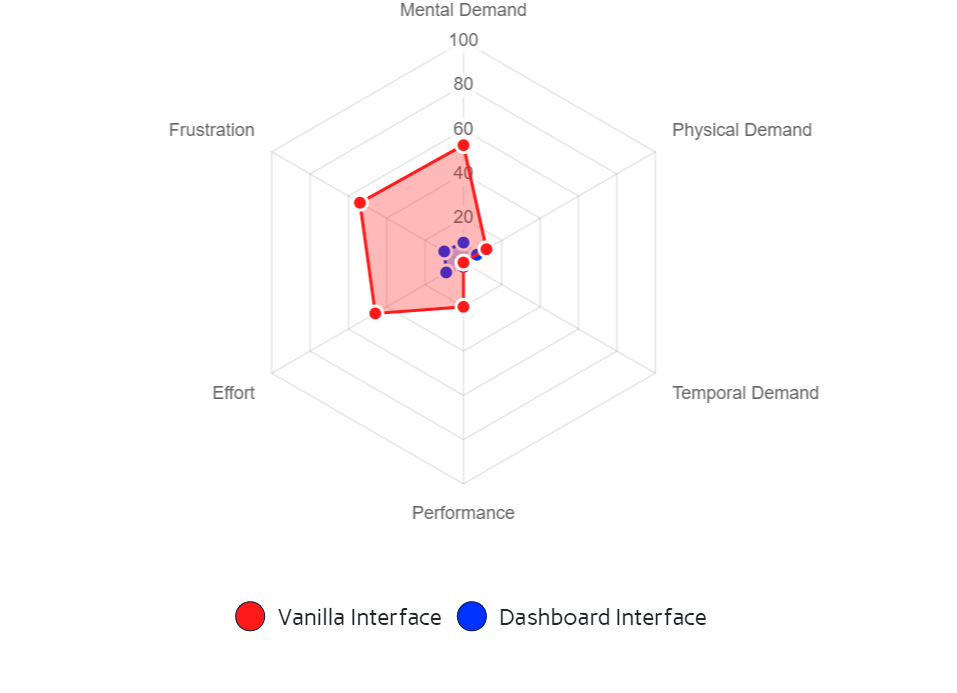
\includegraphics[width=1\textwidth]{Charts/radar-chart.png} 
    \caption{Radar Chart: Visualizing the reduction in multifaceted workload dimensions}
    \label{fig:radchart}
\end{figure}

The most prominent finding is the dramatic contraction of the Dashboard's profile (blue) toward the center of the chart compared to the standard interface (red). 
The standard interface creates a wide, irregular polygon, showing significant peaks in Mental Demand, Effort, and Frustration. In contrast, the Dashboard condition 
collapses these peaks, reducing them to near-minimal levels. This reduction provides empirical evidence that the plugin successfully suppresses Extraneous 
Load while providing the Intrinsic scaffolding necessary to protect the user's finite attentional budget.

\subsection{Efficiency and Time-on-Task Analysis}
The Dashboard demonstrated a large improvement in operational efficiency. As shown in the Table~\ref{tab:time_savings}, users completed configuration
 tasks approximately \textbf{84\% faster} than in the baseline environment.

\begin{table}[h]
\centering
\caption{Comparison of Task Completion Times (Seconds)}
\label{tab:time_savings}
\begin{tabular}{@{}lccc@{}}
\toprule
\textbf{Task} & \textbf{standard Avg (s)} & \textbf{Dashboard Avg (s)} & \textbf{Time Saved} \\ \midrule
Change Theme         & 15.42 & 2.5 & 83.79\% \\
Change Font Size     & 22.10 & 4.2 & 81.00\% \\
Manage Panels* & 32.34 & 3.4 & 89.49\% \\ \bottomrule
\multicolumn{4}{l}{\small \textit{*Note: standard tasks sometimes resulted in incomplete status.}}
\end{tabular}
\end{table}

The ``Manage Panels'' task provided the most striking difference in results. In the standard interface, several participants struggled to locate specific toggle 
settings, leading to a ``search-loop'' behavior. Most of the participants tried to close each panel individually rather than using the ``Customize Layout'' command.
 This resulted in significantly longer completion times and increased frustration and one of the participants giving up completely. 
In the Dashboard, the same task was reduced to a singular, high-visibility interaction therefore the task only took a matter of seconds.

While these timings indicate a clear trend, they should be interpreted with caution. Potential variations in manual timing and the participants'
 varying levels of expertise with the baseline \gls{IDE} (Visual Studio Code) may have influenced the absolute values. 
 Specifically, developers who primarily use alternative editors in their daily workflows may have experienced a steeper learning curve with the ``standard'' interface,
  potentially inflating the initial completion times.


\subsection{SUS Metrics}

The mean SUS score of 92 places the dashboard within the “excellent” usability range, indicating that the interface imposes minimal learnability 
burden and supports rapid user confidence. This is particularly significant within the project context, where reducing onboarding friction and 
preserving attentional continuity were central design goals.

\begin{table}[H]
\centering
\caption{System Usability Scale (SUS) Individual Participant Scores}
\label{tab:sus_results}
\begin{tabular}{lccccccccccc}
\toprule
\textbf{P\#} & \textbf{Q1} & \textbf{Q2} & \textbf{Q3} & \textbf{Q4} & \textbf{Q5} & \textbf{Q6} & \textbf{Q7} & \textbf{Q8} & \textbf{Q9} & \textbf{Q10} & \textbf{Total Score} \\
\midrule
1 & 5 & 1 & 5 & 1 & 5 & 1 & 5 & 1 & 5 & 1 & 100.0 \\
2 & 4 & 2 & 5 & 2 & 4 & 1 & 5 & 1 & 4 & 1 & 87.5 \\
3 & 5 & 1 & 4 & 1 & 5 & 2 & 4 & 1 & 5 & 2 & 90.0 \\
4 & 5 & 1 & 5 & 1 & 5 & 1 & 5 & 2 & 5 & 1 & 97.5 \\
5 & 4 & 2 & 4 & 2 & 4 & 2 & 4 & 1 & 4 & 1 & 85.0 \\
\midrule
\textbf{Avg} & \textbf{4.6} & \textbf{1.4} & \textbf{4.6} & \textbf{1.4} & \textbf{4.6} & \textbf{1.4} & \textbf{4.6} & \textbf{1.2} & \textbf{4.6} & \textbf{1.2} & \textbf{92.0} \\
\bottomrule
\end{tabular}
\end{table}

\subsubsection{Questions 2 \& 6: Complexity and Consistency} 
For developers with \gls{ASD} or \gls{ADHD}, inconsistency is a major source of cognitive strain. If a button moves or a shortcut changes, it can break their focus
entirely. For the dashboard consistency in the design was key, all elements behaved predictably, all buttons were consistent. Your results prove the Dashboard 
provides a stable environment that protects the user`s flow state.

\subsubsection{Questions 4 \& 10: Independence and Learning Curve}
Many \gls{neurodivergent} individuals experience Information Overload when faced with dense manuals or complex onboarding. 
Your score shows the Dashboard is intuitive by design, allowing a developer to begin working immediately without the executive tax of a long learning phase.

\subsubsection{Question 9: Confidence}
Confidence is a massive factor in productivity. By making the interface more intuitive and reducing cognitive load, the Dashboard empowers developers to
feel more in control of their environment, which can lead to increased productivity and job satisfaction.

Overall, even though the results achieved for the Dashboard are excellent, the majority of the participants where people that I know personally or have worked with 
in the past, so there is a potential bias in the results. The next step would be to conduct a larger scale study with a more diverse participant pool to validate 
these findings and ensure they generalise across different populations of developers.

\subsection{Pre-Study Interview Findings}
Prior to the main evaluation, a brief semi-structured interview was conducted with each participant to establish a baseline understanding of their existing 
workflows, coping strategies, and pain points when using traditional \glspl{IDE}. Three dominant themes emerged from the responses.
\begin{itemize}

\item \textbf{Panel Management:} The majority of participants expressed frustration with the number of open panels in a standard \gls{IDE}, yet reported 
that they rarely closed them. Rather than actively managing their workspace, participants described a pattern of passive tolerance, simply ignoring panels 
they did not need. As one participant noted, the effort required to locate and close individual panels felt disproportionate to the benefit, resulting in what 
might be characterised as a ``cognitive acceptance'' of a cluttered environment. This finding directly supports the need for the single-click Minimalist Toggle.


\item \textbf{Task Decomposition:} When asked how they would typically break down a complex programming task, most participants described struggling with initiation.
Several noted that an empty \gls{IDE} felt ``daunting'', and their strategies for overcoming this varied: some wrote rough outlines on paper or 
in a separate document, while others attempted to hold the steps in \gls{working_memory}. One participant reported regularly using ChatGPT to scaffold 
their thinking, but found it tended to generate code directly rather than a structured plan, which they described as ``not helpful for actually getting 
started''. This corroborates the \gls{task_paralysis} literature and provides direct user-grounded motivation for the Task Architect module.

\item \textbf{Error Handling:} Participants consistently reported that cryptic or verbose error messages increased their frustration and interrupted their 
flow. When probed on their typical response to an unfamiliar error, most described a reactive process: attempting solutions from memory, searching 
online, or pasting the error into an AI chatbot. Notably, no participant described a systematic or confident approach to debugging, suggesting that 
the standard \gls{IDE} error output does not provide sufficient \gls{scaffolding} for independent resolution. This reinforces the rationale for the Code Explainer 
module's plain-language feedback approach.

\end{itemize}

\subsection{Real-Time Feedback and User Experience}
During the evaluation, I observed significant differences in how the Dashboard and the standard interface handled real-time feedback. The Dashboard`s capacity to provide instantaneous 
feedback for aesthetic modifications, such as theme and font-size adjustments, where preferred to the baseline interface. This immediate confirmation allowed
 users to acknowledge their actions to system changes instantly, effectively eliminating uncertainty and the associated cognitive load of second-guessing. In 
 contrast, the standard interface`s settings menus often induced ``verification anxiety,'' where users had to manually exit menus to check if a change had 
 been applied. One participant specifically noted that the lack of immediate visual confirmation in the standard \gls{IDE} led to redundant, repetitive attempts, which 
 directly correlated with the higher frustration scores recorded in the NASA-TLX and the higher time taken for these tasks.

Beyond visual configuration, non-visual features such as the AI Task Breakdown and Code Error Checker were evaluated through a ``Think Aloud'' protocol. Participants 
were asked to interact with these features and explain their how they believed that they would work as well has how they could interact with them. From this results were consistently positive,
 all participants accurately identified the functional intent and operational flow of these complex tools.

 For the AI Task Breakdown, a ``manual-vs-automated'' baseline was established. Before triggering the AI, users were asked to verbally outline a high-level 
 decomposition of a programming task. While most provided basic, linear steps, the AI-generated breakdown offered a more granular, comprehensive hierarchical 
 structure. Some participants struggled with breaking down the task manually or needed to write down a plan. Participants reported that having this cognitive 
 \gls{scaffolding} provided directly within the \gls{IDE} served as a significant ``Executive Functioning'' aid. By offloading the mental energy required for task 
 decomposition, a known bottleneck for \gls{neurodivergent} individuals who struggle with initiation and sequencing,
 the Dashboard allowed users to transition into the ``implementation phase'' with less friction.


Similarly, the Code Error Checker transformed the traditionally stressful experience of debugging into an educational interaction. When participants encountered a 
``No File Open'' error, they responded to the Dashboard`s plain-language feedback significantly faster than they did to standard, often cryptic, \gls{IDE} diagnostic messages.
 This reinforces the Dashboard's role not just as a shortcut menu, but as a supportive layer that translates complex system states into actionable information. 
 By providing a safe environment with clear error recovery paths, the system preserves the developer`s ``attentional budget,'' ensuring that minor 
 technical hurdles do not escalate into focus-breaking frustrations. This transition from "system-centric" to "user-centric" feedback is a cornerstone of inclusive 
 design, specifically catering to the need for clarity and predictability in \gls{neurodiverse} workflows.


\subsection{Number of Clicks and User Flow}
The Dashboard's design significantly reduced the number of interactions required to perform common tasks. Changing a theme requires just one click compared to an optimal four in the standard interface.
 It is worth noting that this ``optimal path'' assumes the user already knows exactly where to navigate within VS Code's settings menu, which is often not the case, especially for users who are less 
 familiar with this specific \gls{IDE}.Users unfamiliar with the \gls{IDE} often took a more circuitous route, increasing both click count and completion time beyond the baseline figures reported in Table 7
 Similarly, adjusting font size was reduced to a single Dashboard interaction, eliminating the need to locate and navigate nested editor settings entirely.

The most pronounced difference was observed in panel management. Prior to testing, this was not anticipated to be a significant point of friction; however, it proved to be the task with which participants
 most frequently struggled in the standard condition, with several failing to complete it entirely. Where the standard interface required five or more sequential interactions, varying with the number of open
panels, the Dashboard reduced this to a single toggle. This reduction in interaction depth directly maps to a lower Extraneous Cognitive Load as the developer is no longer required to maintain a mental model
 of the menu hierarchy in \gls{working_memory}, freeing those resources for the primary programming task.

\subsection{Latency Testing}
NFR3 was evaluated by measuring the time for the Dashboard to display the AI-generated task breakdown after the user initiated the request. 
Across all participants, the average latency was 1.8 seconds, with a standard deviation of 0.3 seconds. This meets the requirement that

Maintaining response latency below two seconds is particularly important for \gls{neurodivergent} users, as prolonged waiting periods can disrupt 
attentional continuity and increase the likelihood of task abandonment.



\subsection{Discussion}
The empirical data validates the plugin as a successful ``digital ramp''. 
The 82\% reduction in weighted workload suggests that the ``executive tax'' paid by \gls{neurodivergent} developers
 is not an inherent trait of their neurology, but a byproduct of \gls{neurotypical-bias} in tool design. By suppressing Extraneous Load 
 (via the Minimalist Toggle) and \gls{scaffolding} Intrinsic Load (via the Task Architect), the system maximizes Germane Load, allowing 
 cognitive resources to be redirected toward core algorithmic problem-solving.

\subsection{Limitations}
While the results of this study are encouraging, several limitations must be acknowledged to provide context 
for the findings:
\begin{itemize}
    \item \textbf{Small Sample Size and Recruitment Bias:}
    The study utilized a limited cohort ($N=5$). Furthermore, participants were known to the researcher 
    prior to the study, introducing a potential recruitment bias that may affect the objectivity of the 
    qualitative feedback.
    \item \textbf{Participant Confidentiality and \Gls{neurodiversity} Verification:}
    Due to stringent ethical considerations regarding the storage of sensitive personal data and the project's
     condensed timeline, participants were not explicitly asked to disclose or verify their \gls{neurodivergent} 
     status. Consequently, while the tool is designed for \gls{neurodiverse} profiles, the data cannot be 
     definitively categorized by specific clinical diagnoses.
    \item \textbf{Short-term Evaluation:}
    The experimental tasks were performed in a controlled, short-term setting. Long-term longitudinal
     studies are required to determine if the plugin effectively mitigates ``\gls{hyperfocus} burnout'' or 
     maintains its efficacy over extended, multi-hour work sessions in a professional environment.
    \item \textbf{Baseline Expertise:}
    The absolute values for time-on-task may have been influenced by varying levels of participant expertise
     with the standard VS Code interface. Developers more accustomed to alternative \gls{IDE}s may have experienced
      an inflated learning curve during the standard control phase.
\end{itemize}

\section{Conclusion}
\subsection{Summary of Findings}
This research successfully designed, implemented, and evaluated a VS Code plugin 
tailored to the specific executive functioning needs of neurodivergent software 
developers. The evaluation metrics demonstrate that the ``executive tax'' traditionally
 imposed by industrial IDEs can be significantly mitigated through intentional UI 
 simplification and AI-driven scaffolding

While there where a number of limiting factors I beleve that the research is incurraging.
If I where to contincue to improve the project I would first want to work with neurodiverse people directly
as I feel that I have been having to be very careful in what I could ask participants during the testing.


% 5. References
\printbibliography[heading=bibintoc, title={References}]

\end{document}